\chapter{Phương pháp đề xuất}
\label{sec:related-work}

% Yêu cầu ở preamble: \usepackage{amsmath,amssymb,graphicx}.
% Mặc định biên dịch từ thư mục latex/. Nếu biên dịch từ workspace,
% khối kiểm tra bên dưới tự chọn đường dẫn tương ứng.
\providecommand{\pcrauFigureRoot}{../new/hinhanh}
\IfFileExists{new/hinhanh/04_language_query_graph/fig04_language_query_graph_v2.pdf}{%
  \renewcommand{\pcrauFigureRoot}{new/hinhanh}}{}

Chương này trình bày phương pháp P-CRA-U
(\emph{Probabilistic Cross-modal Relation-Aware Uncertainty}) cho bài toán
grounding thị giác--ngôn ngữ có quan hệ không gian. Điểm xuất phát là mô hình
RoboRefer-2B-SFT đã được huấn luyện trước; đóng góp của hệ thống nằm ở nhánh
bổ sung biểu diễn truy vấn, dự đoán phân bố vị trí và đánh giá khả năng trả lời,
sau đó hiệu chuẩn rủi ro để đưa ra quyết định chọn lọc.
Nội dung mô tả nền sidecar V2 và bước Adapter answerability của phiên bản P-CRA-U được chọn. Các khối RGB-D, query graph, spatial, edge và source kế thừa V2 đóng băng; chỉ Adapter học thêm tham số, rồi risk được hiệu chuẩn lại. Chương này tập
trung vào cơ chế và mục tiêu học; Chương~4 ghi cấu hình cùng quy trình
chọn checkpoint, còn Chương~5 đánh giá hiệu quả. Thành phần mở rộng
trong pipeline được phân biệt với đường xử lý đã hiện thực.

\section{Tổng quan hệ thống}
\label{sec:method-overview}

\subsection{Mục tiêu và nguyên tắc thiết kế}

Với một ảnh RGB, một ảnh depth và một câu lệnh, mô hình grounding thông
thường trả về một điểm trên ảnh. Tuy nhiên, một điểm đơn lẻ không cho biết
câu lệnh có nhiều ứng viên, vật đích không tồn tại, hay ảnh hiện tại thiếu
bằng chứng do che khuất và chất lượng depth. Vì vậy, phương pháp đề xuất
không chỉ tìm vị trí có điểm số lớn nhất, mà còn trả lời câu hỏi:
\emph{bằng chứng hiện tại có đủ để chấp nhận vị trí này hay không?}

Hệ thống được xây dựng theo ba nguyên tắc. Thứ nhất, giữ nguyên mô hình
nền để bảo toàn đường suy luận RoboRefer và tạo điều kiện so sánh với
baseline \cite{zhou2025roborefer,roborefer2bsftModelCard}. Thứ hai, tách dự
đoán vị trí khỏi đánh giá khả năng trả lời: ngay cả khi heatmap có một đỉnh
rõ, câu lệnh vẫn có thể thuộc lớp \texttt{ABSENT}. Thứ ba, không đồng nhất
điểm số của mạng với xác suất lỗi; rủi ro grounding phải được ước lượng
qua một bộ hiệu chuẩn độc lập.

\paragraph{Ý tưởng thiết kế và hai đóng góp phương pháp.}
Đóng góp thứ nhất là sidecar đa nhiệm có điều kiện theo truy vấn:
cùng một biểu diễn RGB-D--ngôn ngữ tạo phân bố vị trí, evidence
đích--vật mốc--quan hệ, answerability và score nguồn. Thiết kế cho phép
giữ thông tin về các vùng ứng viên đồng thời dự đoán điều kiện trả lời.
Đóng góp thứ hai là bước hiệu chuẩn độc lập sau freeze, liên kết evidence
với biến cố lỗi nhận thức rồi chọn quyết định theo risk. Vùng không gian
là đầu ra riêng được đánh giá cùng coverage--area.

Các cơ chế query slots, fusion, head đa nhiệm và logistic calibration
được tổ chức thành một phương pháp triển khai thống nhất. Đây là ý tưởng
kết hợp của khóa luận; việc thành phần xuất hiện trong kiến trúc chưa
chứng minh lợi ích riêng của thành phần đó. So sánh toàn hệ thống và
ablation có vai trò khác nhau trong kiểm chứng giả thuyết thiết kế.

\subsection{Các khối chức năng và luồng dữ liệu}

Kiến trúc mục tiêu gồm bảy khối: đầu vào đa phương thức; mã hóa và
hợp nhất RGB--depth--ngôn ngữ; backbone RoboRefer; biểu diễn truy vấn quan
hệ; sidecar P-CRA-U; chính sách quyết định chọn lọc; và môi trường kiểm
chứng. Bộ hiệu chuẩn nằm giữa sidecar và chính sách quyết định.
Hình~\ref{fig:method-pipeline} biểu diễn tổng thể kiến trúc này.

\begin{figure}[htbp]
    \centering
    \IfFileExists{../plan/pipeline.png}{%
        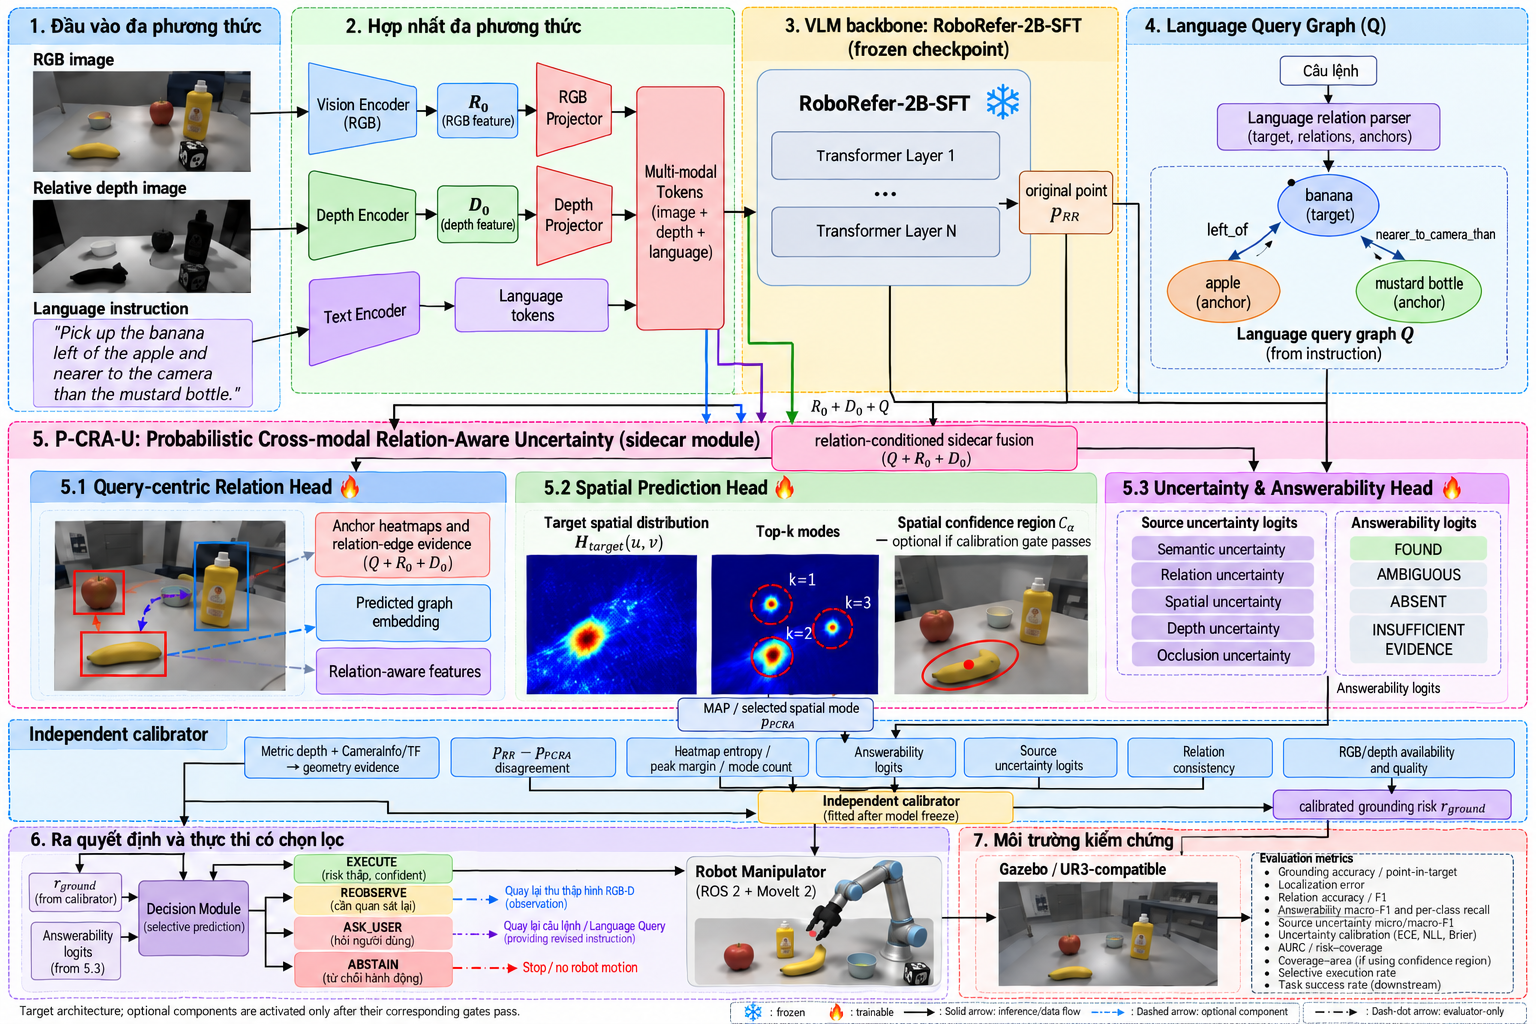
\includegraphics[width=\textwidth,height=0.78\textheight,keepaspectratio]{hinhanh/pipeline.png}
    }{%
        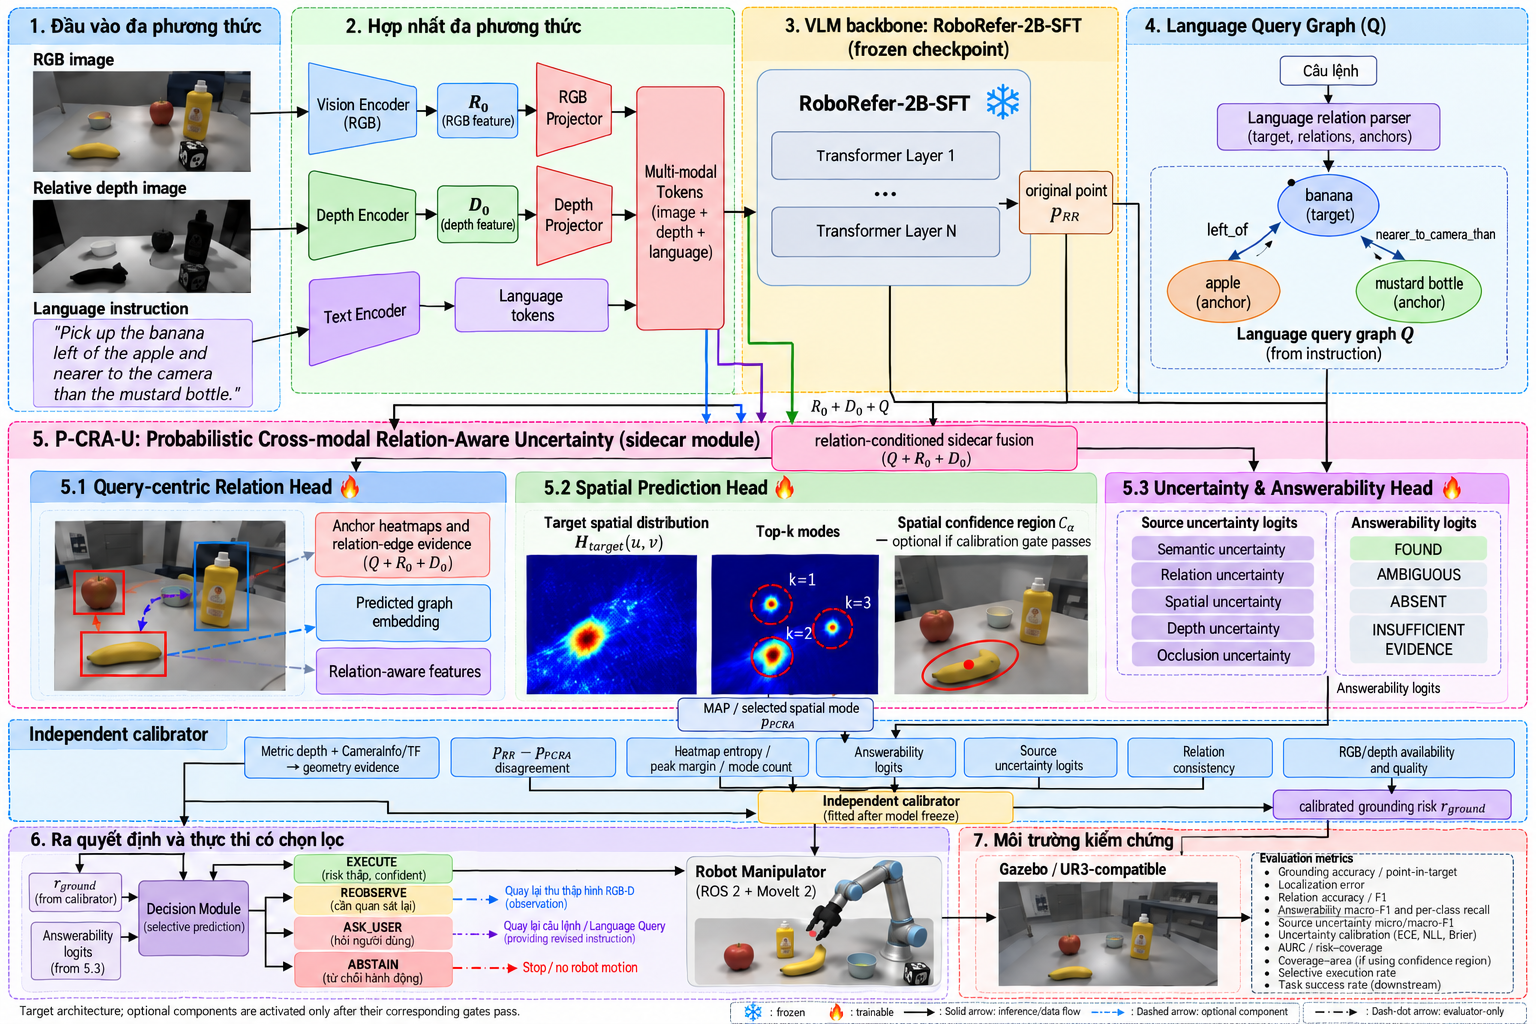
\includegraphics[width=\textwidth,height=0.78\textheight,keepaspectratio]{hinhanh/pipeline.png}
    }
    \caption{Kiến trúc mục tiêu của hệ thống grounding có quan hệ và bất định.
    Sơ đồ mô tả cả thành phần đã triển khai và thành phần mở rộng; các khác
    biệt của V2 được giải thích trong nội dung chương.}
    \label{fig:method-pipeline}
    {\footnotesize Nguồn: sơ đồ thiết kế do tác giả xây dựng, tệp
    \texttt{plan/pipeline.png} trong workspace.\par}
\end{figure}

Trong V2, đường dữ liệu cốt lõi được viết dưới dạng
\begin{align}
    (R_0,D_0)&=\mathcal{E}_{\theta_{RR}}(I,Z_{\mathrm{rel}}),\\
    Q&=\mathcal{Q}_{\theta_Q}(q),\\
    \mathcal{O}&=\mathcal{S}_{\theta_S}(R_0,D_0,Q),\\
    r_{\mathrm{ground}}&=C_{\phi}(e(\mathcal{O})),\\
    a&=\pi(r_{\mathrm{ground}},p_{\mathrm{ans}},p_{\mathrm{src}}).
\end{align}
Ở đây, $\mathcal{E}$ là các tower đặc trưng đóng băng của RoboRefer;
$\mathcal{Q}$ là bộ mã hóa truy vấn của sidecar; $\mathcal{S}$ là các
khối fusion và các head dự đoán; $e$ là vector bằng chứng; và $a$ là một
trong bốn quyết định. Điểm gốc $p_{RR}$ được tính bằng đường suy luận
RoboRefer riêng khi cần so sánh hoặc xây dựng đặc trưng bất đồng.

Một khác biệt cần lưu ý là sidecar V2 lấy đặc trưng trước projector từ
hai tower, không lấy trạng thái ẩn của các lớp ngôn ngữ cuối cùng trong
RoboRefer. Bộ mã hóa câu lệnh của sidecar cũng là một mạng riêng.
Do đó, sơ đồ mục tiêu không nên được diễn giải thành việc mọi mũi tên
từ backbone đến sidecar đều đã được hiện thực hóa bằng cùng một loại tensor.

Về vận hành, suy luận gồm ba bước: mã hóa RGB/depth bằng tower đóng băng
và mã hóa câu lệnh bằng mạng sidecar; fusion cùng các head dự đoán tạo
evidence và điểm MAP; calibrator/policy cố định tạo risk, region và
decision. Mask target, anchor và nhãn chuẩn chỉ xuất hiện trong giám sát,
fit calibration hoặc evaluator, không nằm trên đường suy luận nhận thức.

\subsection{Đầu ra và phạm vi kiểm chứng}

Đầu ra $\mathcal{O}$ gồm logits vị trí target, interior và anchor; logits
cạnh quan hệ; logits answerability; logits của năm nguồn uncertainty;
cùng một số đặc trưng fusion. Sau xử lý, hệ thống tạo heatmap chuẩn hóa,
điểm MAP, các mode không gian, rủi ro và quyết định.

Phạm vi bằng chứng được chia theo chức năng. Grounding MAP, answerability,
source, edge proxy, risk, region và policy đã có đánh giá Test-IID.
Anchor heatmap và các mode đã có đường dự đoán/hậu xử lý, nhưng chưa có
bộ metric anchor hoặc instance/top-$k$ đầy đủ. Kiểm tra RGB-D độc lập và
ổn định nhiều frame đã có audit demo; gate hình học đầy đủ và handoff
MoveIt chưa được tích hợp vào policy V2 đã xác minh.

Ở phần mô phỏng, \texttt{EXECUTE} nghĩa là \emph{chấp nhận grounding theo
policy}. Kiểm chứng thao tác còn cần back-projection 3D đúng TF,
reachability, va chạm, tư thế gắp và trạng thái vật sau hành động.

\section{Đầu vào đa phương thức}
\label{sec:method-input}

\subsection{Ảnh RGB, depth và câu lệnh}

Một mẫu quan sát được ký hiệu
\begin{equation}
    x=(I,Z_{\mathrm{rel}},q),\qquad
    I\in\mathbb{R}^{H\times W\times3},\quad
    Z_{\mathrm{rel}}\in\mathbb{R}^{H\times W}.
\end{equation}
Với dữ liệu hiện tại, ảnh có kích thước $H=480$, $W=640$.
Câu lệnh $q=(w_1,\ldots,w_n)$ mô tả vật đích trực tiếp hoặc thông qua
quan hệ với các vật mốc. Ảnh RGB và depth cần cùng kích thước và có
đăng ký tương ứng theo pixel; nếu không, đặc trưng depth tại một ô
không còn mô tả vùng RGB tương ứng.

Trong mô phỏng, ngoài đầu vào mạng, hệ thống có thể lưu
$Z_{\mathrm{metric}}$ theo mét, ma trận nội tại $K$ và phép biến đổi
$T_{\mathrm{base}\leftarrow\mathrm{camera}}$.
Các đại lượng này phục vụ hình học ở Mục~\ref{sec:method-3d};
chúng không nằm trong tập input của sidecar V2.

\subsection{Phân biệt relative depth và metric depth}

Relative depth biểu diễn cấu trúc gần--xa phù hợp với tower depth.
Metric depth biểu diễn khoảng cách vật lý để suy ngược điểm 3D.
Không thể thay thế hai loại depth cho nhau: ảnh 8-bit đã chuẩn hóa
không còn giữ trực tiếp thang đo mét.

Trong quy trình capture hiện có, tập pixel depth hợp lệ là
\begin{equation}
    \mathcal{V}=\{(u,v): Z_{\mathrm{metric}}(u,v)
    \text{ hữu hạn},\ 0.10\leq Z_{\mathrm{metric}}(u,v)\leq2.0\}.
\end{equation}
Đặt $z_{\mathrm{near}}$ và $z_{\mathrm{far}}$ là các phân vị 2\% và
98\% trên $\mathcal{V}$. Sau khi chặn depth vào khoảng này, giá trị
relative depth được tính bằng
\begin{equation}
    Z_{\mathrm{rel}}(u,v)=255\,
    \operatorname{clip}_{[0,1]}
    \left(
    \frac{1/\widetilde{z}(u,v)-1/z_{\mathrm{far}}}
         {1/z_{\mathrm{near}}-1/z_{\mathrm{far}}}
    \right).
    \label{eq:method-relative-depth}
\end{equation}
Pixel không hợp lệ được gán 0; ảnh xám được lặp thành ba kênh cho
đường tiền xử lý depth. Nếu khoảng phân vị suy biến, quy trình thử
khoảng min--max; nếu vẫn không có khoảng depth sử dụng được hoặc có
quá ít pixel hợp lệ, capture không được chấp nhận.

\subsection{Ranh giới giữa quan sát và nhãn}

Mask vật đích, mask anchor, nhãn answerability, nhãn source và thông
tin audit của cảnh chỉ phục vụ tạo supervision hoặc đánh giá.
Chúng không được đưa vào hàm forward. Trong code, tập khóa đầu vào
được giới hạn tường minh ở các đặc trưng RGB/depth, đặc trưng thumbnail,
token, relation ID và các mask cấu trúc suy ra từ câu lệnh.
Khóa ngoài tập này làm phát sinh lỗi.

Cách tổ chức trên giúp ngăn rò rỉ nhãn qua giao diện mô hình. Tuy nhiên,
đây chỉ là một lớp bảo vệ kỹ thuật; dữ liệu, cache và quy trình chia
family vẫn phải được kiểm tra độc lập để bảo đảm không có ảnh hoặc
biến thể cùng family bị dùng chéo giữa các tập đánh giá.

\section{Trích xuất đặc trưng đa phương thức}
\label{sec:method-features}

\subsection{Đặc trưng trước projector của RoboRefer}

Gọi $E_{\mathrm{rgb}}$ và $E_{\mathrm{depth}}$ là các tower đóng băng:
\begin{equation}
    R_{\mathrm{raw}}=E_{\mathrm{rgb}}(I),\qquad
    D_{\mathrm{raw}}=E_{\mathrm{depth}}(Z_{\mathrm{rel}}).
\end{equation}
Đặc trưng lấy trước projector giữ không gian biểu diễn của tower và
cho phép sidecar học phép chiếu riêng. Với cấu hình tiền xử lý đang
được khóa, mỗi phương thức tạo tensor
\begin{equation}
    R_{\mathrm{raw}},D_{\mathrm{raw}}
    \in\mathbb{R}^{13\times1024\times1152}.
\end{equation}
Mười hai tile cục bộ được bố trí thành ba hàng, bốn cột;
mỗi tile có lưới token $32\times32$. Tile thứ mười ba là thumbnail
toàn ảnh. Hàm pooling kiểm tra đúng shape này thay vì tự giả định
các cấu hình dynamic tiling khác cũng tương thích.

\subsection{Tái lập lưới đặc trưng toàn ảnh}

Mỗi tile cục bộ được average pooling với kernel và stride bằng 4,
từ $32\times32$ xuống $8\times8$. Ghép các tile theo vị trí cho lưới
\begin{equation}
    R_0,D_0\in\mathbb{R}^{24\times32\times1152}.
    \label{eq:method-feature-shape}
\end{equation}
Layer normalization được áp dụng theo chiều đặc trưng 1152.
Vì vậy, lưới $32\times32$ trong mô tả tower là lưới của \emph{một tile},
không phải lưới cuối cùng của sidecar V2.

Thumbnail được lấy trung bình trên 1024 token rồi chuẩn hóa:
\begin{equation}
    r_{\mathrm{thumb}}=
    \operatorname{LN}\left(\frac{1}{1024}
    \sum_i R_{\mathrm{raw}}^{(13)}(i)\right),
    \qquad
    d_{\mathrm{thumb}}=
    \operatorname{LN}\left(\frac{1}{1024}
    \sum_i D_{\mathrm{raw}}^{(13)}(i)\right).
\end{equation}
Hai vector này bổ sung bối cảnh toàn cảnh cho các head phân loại.

\subsection{Cache đặc trưng và tính nhất quán}

Do tower đóng băng, các đặc trưng có thể được tính trước và lưu cache
để huấn luyện sidecar mà không chạy lại backbone ở từng epoch.
Cache phải gắn với đúng ảnh, depth, checkpoint tower và cấu hình
tiền xử lý. Đổi cách chuẩn hóa depth hoặc thứ tự tile sẽ làm đầu vào
khác với đầu vào đã dùng để huấn luyện dù kích thước tensor vẫn giống nhau.

Khi suy luận trực tiếp từ camera, cần tái dùng cùng quy trình tiền xử lý,
pooling và chuẩn hóa. Việc có ảnh RGB-D hợp lệ từ ROS chưa đủ để khẳng
định đã khớp miền dữ liệu huấn luyện; góc camera, bố cục vật thể và
chất lượng depth vẫn có thể làm thay đổi phân bố đặc trưng.

\section{Backbone RoboRefer-2B-SFT đóng băng}
\label{sec:method-backbone}

\subsection{Vai trò của đường grounding gốc}

RoboRefer được giữ như mô hình nền chuyên biệt cho grounding không gian
\cite{zhou2025roborefer}. Ở mức khái niệm, ảnh, depth và token ngôn ngữ
được chiếu vào không gian đa phương thức:
\begin{equation}
    X_{RR}=[P_R(R_{\mathrm{raw}});
    P_D(D_{\mathrm{raw}});L_{RR}],
    \qquad
    p_{RR}=\mathcal{G}_{\theta_{RR}}(X_{RR}).
\end{equation}
Đây là biểu diễn tóm tắt, không phải khẳng định chi tiết thứ tự token
và prompt template bên trong implementation. Khi chạy baseline,
đường tiền xử lý và suy luận gốc được giữ riêng với sidecar.

\subsection{Tách tham số mô hình nền và tham số học mới}

Trong huấn luyện V2,
\begin{equation}
    \theta_{RR}=\mathrm{constant},\qquad
    \theta_S=\{\theta_Q,\theta_{\mathrm{fusion}},
    \theta_{\mathrm{spatial}},\theta_{\mathrm{edge}},
    \theta_{\mathrm{ans}},\theta_{\mathrm{src}}\}
\end{equation}
là tập tham số được tối ưu. Bộ hiệu chuẩn $\phi$ được fit sau khi
checkpoint sidecar đã được chọn và đóng băng.

Thiết kế này giảm chi phí huấn luyện và tránh làm thay đổi baseline.
Đổi lại, sidecar không thể sửa trực tiếp những biểu diễn mà tower
chưa mã hóa tốt. Hiệu quả của phương pháp cần được đánh giá trên cùng
ảnh và cùng câu lệnh với RoboRefer gốc, không suy ra chỉ từ loss của
sidecar.

\subsection{Vai trò của điểm RoboRefer trong V2}

$p_{RR}$ không phải đầu vào trực tiếp của mạng sidecar. Điểm này
được sử dụng để so sánh grounding và có thể tạo đặc trưng bất đồng
cho bộ hiệu chuẩn. Như vậy, heatmap V2 không chỉ là một vùng vẽ quanh
$p_{RR}$; nó được dự đoán từ đặc trưng RGB-D và truy vấn riêng.
Nếu không có điểm RoboRefer, sidecar vẫn tạo được dự đoán, còn bộ
hiệu chuẩn ghi nhận trạng thái thiếu đặc trưng này.

\section{Biểu diễn truy vấn quan hệ Language Query Graph}
\label{sec:method-query-graph}

\subsection{Đồ thị khái niệm và biểu diễn vận hành}

Ở mức ngữ nghĩa, truy vấn gồm một vật đích, các quan hệ và các vật mốc:
\begin{equation}
    Q=(V,E),\qquad
    V=\{v_t,v_{a_1},\ldots,v_{a_K}\}.
\end{equation}
Ví dụ, câu “Pick up the banana left of the apple and nearer to the
camera than the mustard bottle” có thể được phân tích thành target
banana, anchor apple với quan hệ \texttt{left\_of}, và anchor mustard
bottle với quan hệ gần camera hơn.

Tuy nhiên, V2 không có một parser ngữ nghĩa hoàn chỉnh trả về tên noun
được ràng buộc chính xác với từng cạnh. Biểu diễn vận hành gồm token
câu lệnh, ID quan hệ tìm bằng mẫu chuỗi, và các query slot học được.
Sự tương ứng giữa slot và vùng ảnh được học từ supervision, thay vì
có một bộ nhận dạng vật thể cố định cấp trực tiếp tên node.

\subsection{Nhận diện quan hệ và mask cấu trúc}

Tập quan hệ đang dùng là
\begin{equation}
\begin{split}
    \mathcal{R}=\{&
    \texttt{direct},\texttt{left\_of},\texttt{right\_of},
    \texttt{front\_of},\texttt{behind},\\
    &\texttt{nearer\_than},\texttt{farther\_than},
    \texttt{between\_in\_depth},\texttt{nearer\_than\_both}\}.
\end{split}
\end{equation}
Bộ nhận diện tìm lần khớp đầu tiên cho từng loại, sắp xếp theo vị trí
trong câu, loại trùng và giữ tối đa ba relation slot. Khi nhận diện
\texttt{nearer\_than\_both}, quan hệ \texttt{nearer\_than} chung được bỏ
để tránh đếm kép. Nếu không tìm thấy quan hệ, lớp \texttt{direct}
được dùng.

Số anchor slot hoạt động được xác định bằng quy tắc: truy vấn trực
tiếp có 0 anchor; truy vấn chứa \texttt{between\_in\_depth} hoặc
\texttt{nearer\_than\_both} có 2 anchor; các trường hợp còn lại dùng
số quan hệ, tối đa 3. Đây là heuristic phù hợp với bộ mẫu câu hiện
tại, không phải bộ suy luận tổng quát cho mọi cấu trúc ngôn ngữ.

Hai mask $m_l^{r}$ và $m_k^{a}$ chỉ biểu diễn slot được kích hoạt
từ câu lệnh. Đặc biệt, $m_k^{a}=1$ không chứng minh anchor đang
hiện diện hoặc nhìn thấy rõ trong ảnh.

\subsection{Minh họa bằng trường hợp thực tế}

Hình~\ref{fig:method-query-graph} thể hiện đúng đường xử lý V2:
token câu lệnh được contextualize, các relation ID bổ sung điều kiện
cho query slot, sau đó target, relation và anchor slot được tạo ra.
Các nhãn node trong minh họa phục vụ giải thích câu lệnh; không được
hiểu là đầu ra của một noun parser độc lập đã được kiểm chứng.

\begin{figure}[htbp]
    \centering
    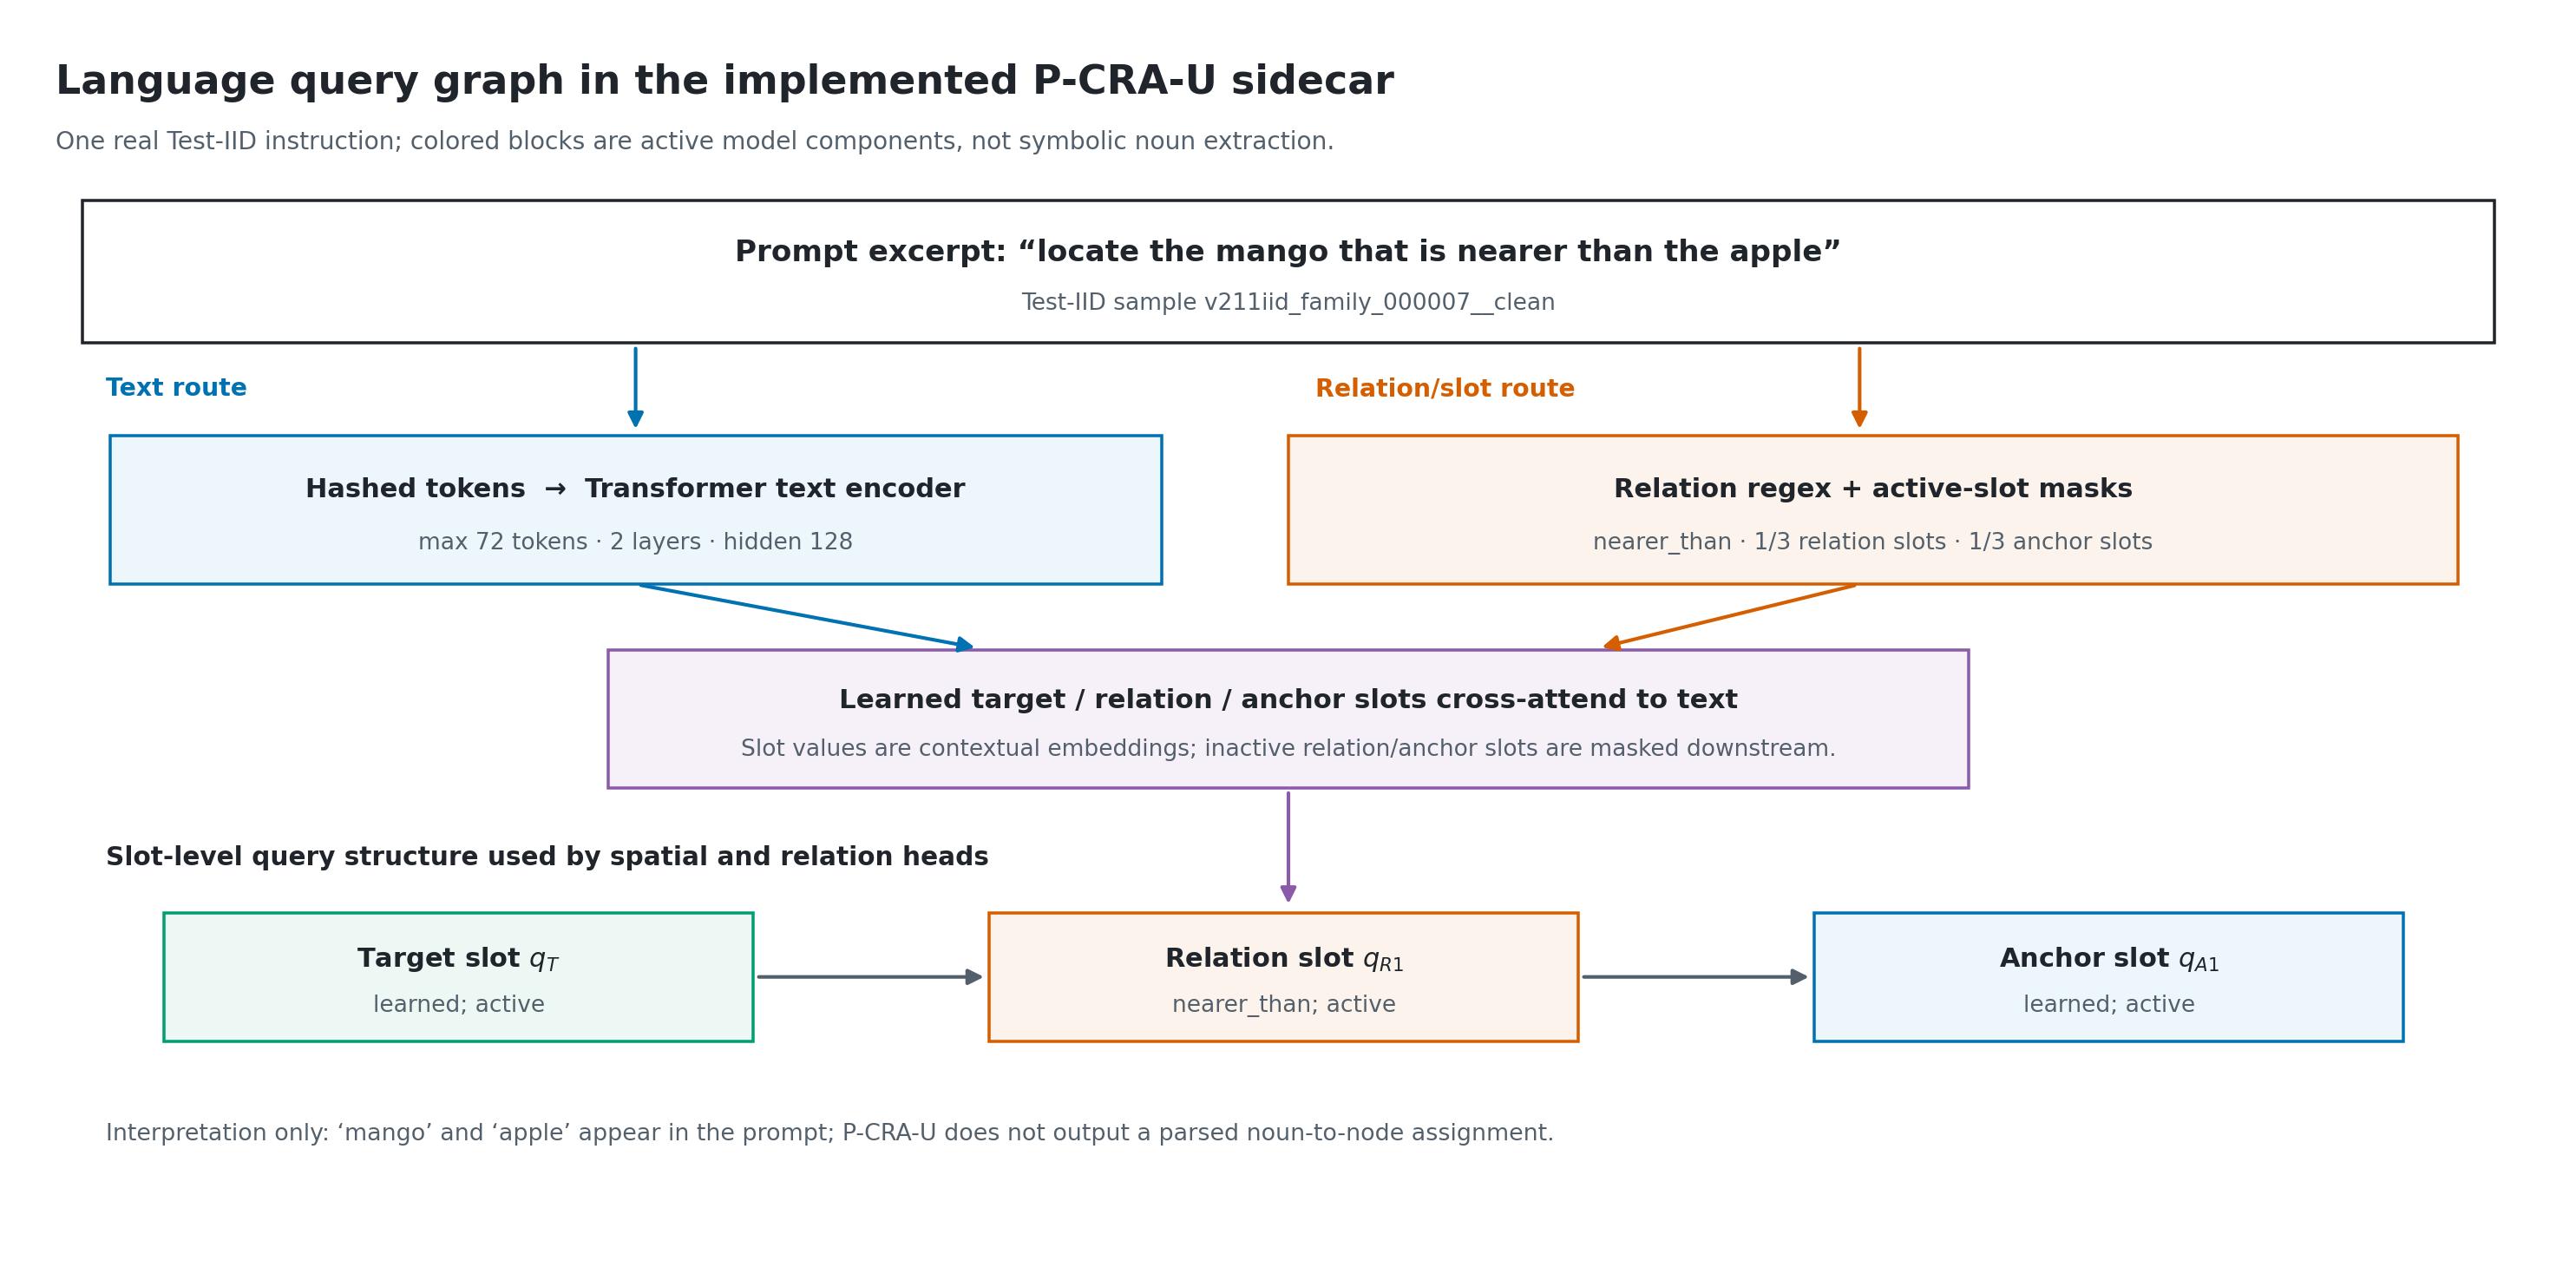
\includegraphics[width=\textwidth]{hinhanh/fig04_language_query_graph_v2.png}
    \caption{Biểu diễn truy vấn quan hệ trong implementation V2.
    Hình dựng từ một câu lệnh thực trong dữ liệu, minh họa các query
    slot và mask cấu trúc thay vì một scene graph ground-truth.}
    \label{fig:method-query-graph}
    {\footnotesize Nguồn: tác giả dựng từ bộ mã hóa câu lệnh và mô hình
    V2 trong workspace; minh họa với mẫu
    \texttt{v211iid\_family\_000007\_\_clean}.\par}
\end{figure}

\section{Bộ trích xuất truy vấn có ngữ cảnh}
\label{sec:method-contextual-query}

\subsection{Token hóa và mã hóa câu lệnh}

Bộ token hóa riêng của sidecar chuẩn hóa câu lệnh tiếng Anh và ánh xạ
token bằng hashing vào bảng embedding. Padding được tách bằng mask;
chi tiết ánh xạ và giới hạn chuỗi được ghi ở Chương~4. Đây là biểu diễn
văn bản học trong sidecar, có khả năng va chạm hash và giới hạn miền mẫu
câu, cần phân biệt với tokenizer pretrained của RoboRefer.

Đặt $d=128$. Embedding token và vị trí được cộng trước khi đưa vào
Transformer:
\begin{equation}
    L=\operatorname{Transformer}_{2}
    \bigl(E_{\mathrm{tok}}(\operatorname{id}(q))+E_{\mathrm{pos}}\bigr)
    \in\mathbb{R}^{n\times d}.
\end{equation}
Encoder có hai lớp, bốn attention head, feed-forward rộng $4d$,
GELU, pre-normalization và dropout 0.1. Padding được loại bằng
attention mask. Cơ chế contextualization kế thừa nguyên lý attention
trên chuỗi \cite{vaswani2017attention}, nhưng các tham số ở đây được
học trong sidecar.

\subsection{Query slot và cross-attention với văn bản}

Mạng có một target slot, ba relation slot và ba anchor slot.
Các vector khởi tạo đều là tham số học được. Relation slot còn nhận
embedding ID quan hệ:
\begin{equation}
    U=[u_t;\ u_{r_1}+E_r(r_1);\ldots;u_{r_3}+E_r(r_3);
    \ u_{a_1};\ldots;u_{a_3}]\in\mathbb{R}^{7\times d}.
\end{equation}
Các slot truy vấn văn bản thông qua multi-head attention:
\begin{equation}
    Q_{\mathrm{slot}}=
    \operatorname{LN}\bigl(U+\operatorname{MHA}(U,L,L)\bigr).
    \label{eq:method-query-slots}
\end{equation}
Đầu ra được tách thành $q_t$, $\{q_{r_l}\}_{l=1}^{3}$ và
$\{q_{a_k}\}_{k=1}^{3}$. Cross-attention ở bước này là
\emph{slot--văn bản}, không phải attention trực tiếp giữa slot và
lưới RGB-D.

\subsection{Vector bối cảnh}

Vector quan hệ và văn bản toàn cục được tính bằng masked mean:
\begin{equation}
    c_r=\frac{\sum_l m_l^r q_{r_l}}{\max(1,\sum_l m_l^r)},\qquad
    c_q=\frac{\sum_j m_j^{\mathrm{tok}} L_j}
    {\max(1,\sum_j m_j^{\mathrm{tok}})}.
\end{equation}
$c_r$ điều kiện hóa fusion; $c_q$ tham gia các head phân loại.
Với truy vấn \texttt{direct}, relation slot tương ứng vẫn hoạt động
để cung cấp ngữ cảnh, nhưng không có anchor và cạnh quan hệ hữu hiệu.

\section{Hợp nhất RGB-D có điều kiện quan hệ}
\label{sec:method-fusion}

\subsection{Chiếu đặc trưng và tạo modality gate}

Tại mỗi ô $i$ của lưới $24\times32$, hai đặc trưng 1152 chiều được
chiếu tuyến tính về $d=128$:
\begin{equation}
    r_i=W_R R_{0i},\qquad d_i=W_D D_{0i},\qquad
    j_i=[r_i;d_i;c_r]\in\mathbb{R}^{3d}.
\end{equation}
Các phép chiếu RGB và depth không dùng bias. Modality gate được tính bằng
\begin{equation}
    g_i=\sigma\bigl(\operatorname{MLP}_g(j_i)\bigr)
    \in(0,1)^d,
    \label{eq:method-modality-gate}
\end{equation}
trong đó $\operatorname{MLP}_g$ gồm hai lớp tuyến tính
$3d\rightarrow d\rightarrow d$ với GELU ở giữa.
Gate là vector theo kênh tại từng ô, không phải một giá trị
xác suất duy nhất của độ tin cậy depth.

\subsection{Nhánh tương tác và các khối residual}

Nhánh tương tác đa phương thức là một MLP khác có cùng cấu trúc:
\begin{equation}
    F_i^{(0)}=
    \operatorname{LN}\bigl(
    r_i+g_i\odot d_i+\operatorname{MLP}_{\mathrm{cross}}(j_i)
    \bigr).
    \label{eq:method-fusion}
\end{equation}
Nhánh này nhận đồng thời RGB, depth và điều kiện quan hệ, nhưng
\emph{không phải} một lớp relation-conditioned attention.
Hai khối residual MLP tiếp tục biến đổi đặc trưng:
\begin{equation}
    F^{(b+1)}=
    F^{(b)}+
    W_2^{(b)}
    \operatorname{Dropout}
    \left(\operatorname{GELU}\bigl(W_1^{(b)}
    \operatorname{LN}(F^{(b)})+b_1^{(b)}\bigr)\right)
    +b_2^{(b)},\quad b=0,1,
\end{equation}
với nhánh ẩn rộng $2d$. Kết quả cuối là
$F\in\mathbb{R}^{24\times32\times128}$.

\subsection{Ý nghĩa và giới hạn}

Một câu hỏi về gần--xa có thể cần sử dụng depth khác với câu hỏi về
vị trí trái--phải. Điều kiện $c_r$ cho phép gate và nhánh tương tác
thích nghi với loại truy vấn. Tuy nhiên, gate lớn không chứng minh
depth đúng, và gate nhỏ không tự chứng minh depth hỏng; đây là
trọng số học được bên trong mô hình.

Hình~\ref{fig:method-fusion} minh họa tensor và các nhánh đúng theo code.
Dropout trong các residual block của baseline V2 là 0.1.
Modality dropout bổ sung trong experiment V3 không được coi là thành
phần đã kích hoạt khi mô tả checkpoint V2 epoch 13.

\begin{figure}[htbp]
    \centering
    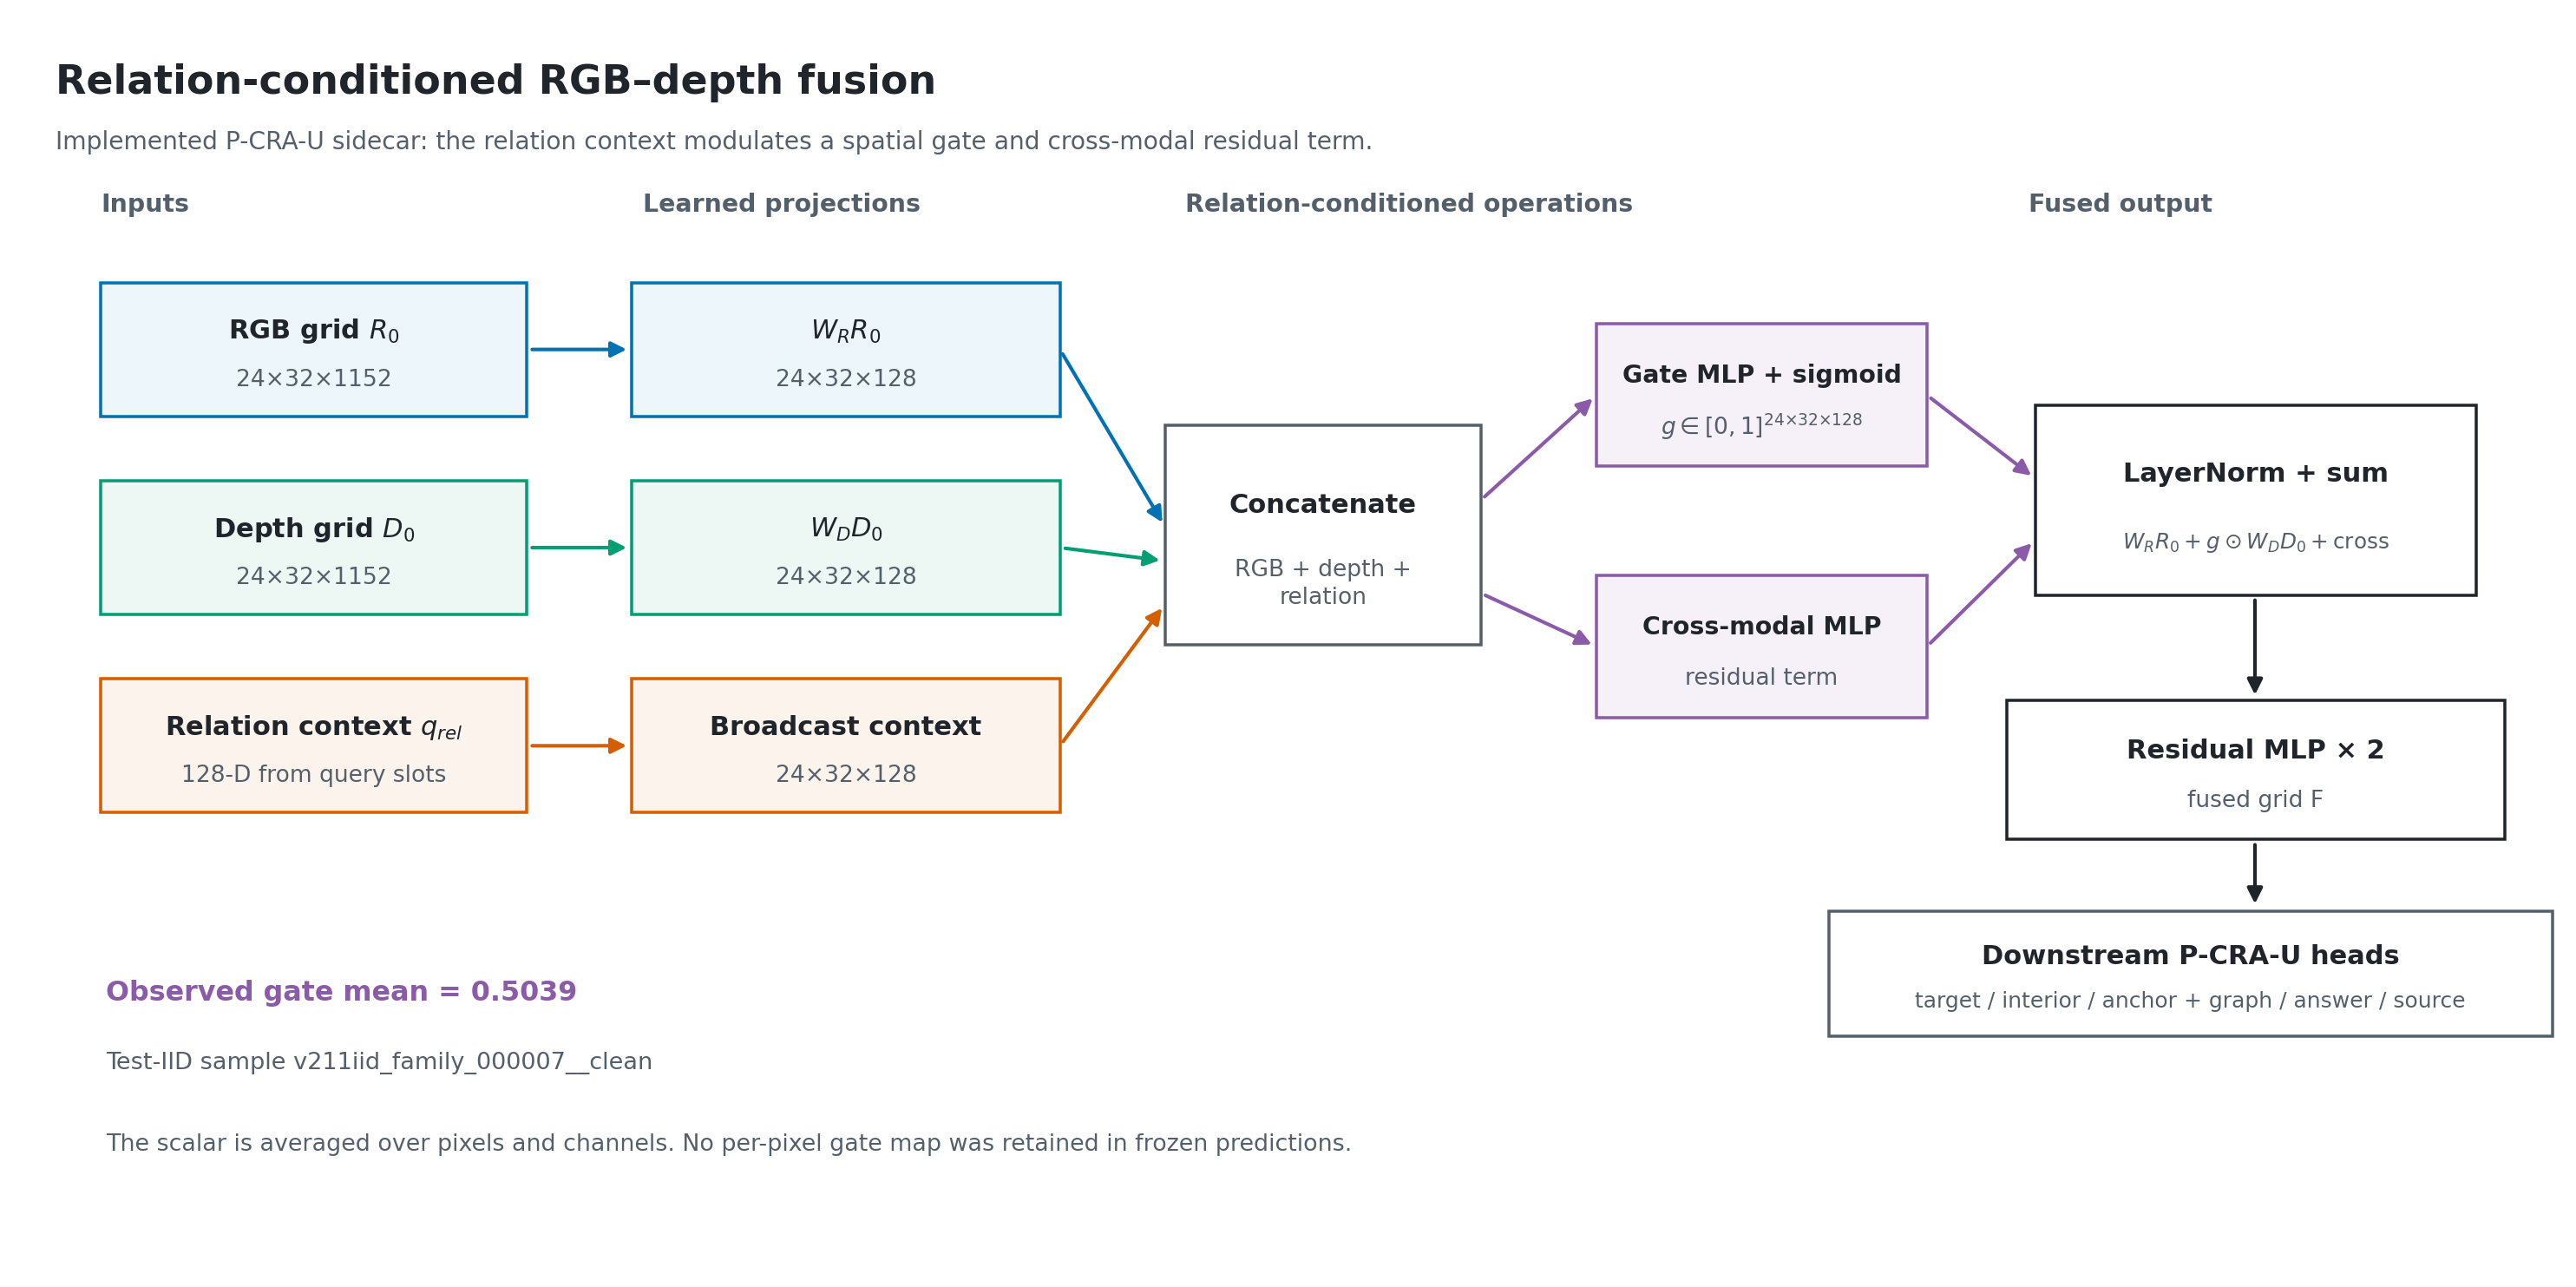
\includegraphics[width=\textwidth]{hinhanh/fig05_relation_conditioned_fusion_v2.png}
    \caption{Hợp nhất RGB-D có điều kiện quan hệ trong V2:
    phép chiếu đặc trưng, gate theo kênh, nhánh tương tác MLP và hai
    residual MLP. Giá trị gate trong minh họa là thống kê của một
    prediction thực, không phải bản đồ chất lượng cảm biến.}
    \label{fig:method-fusion}
    {\footnotesize Nguồn: tác giả dựng từ cấu trúc
    \texttt{RelationConditionedFusion} và dữ liệu suy luận V2 trong workspace.\par}
\end{figure}

\section{Nhánh quan hệ tập trung vào truy vấn}
\label{sec:method-relation-head}

\subsection{Dự đoán các vùng anchor}

Với query anchor $q_{a_k}$, head không gian dùng tương tác tích vô hướng
giữa đặc trưng thị giác và query:
\begin{equation}
    \ell_{a_k,i}=
    \frac{(W_v^a F_i+b_v^a)^{\mathsf T}
    (W_q^a q_{a_k}+b_q^a)}{\sqrt{d}}
    +b_a(q_{a_k}).
    \label{eq:method-anchor-logit}
\end{equation}
$b_a$ là phép chiếu tuyến tính từ query về một scalar.
Các anchor slot dùng chung tham số spatial head, nhưng query khác nhau.
Phân bố node anchor được chuẩn hóa trên toàn bộ $N_g=24\times32=768$ ô:
\begin{equation}
    H_{a_k,i}=
    \frac{\exp(\ell_{a_k,i})}
    {\sum_{j=1}^{N_g}\exp(\ell_{a_k,j})}.
\end{equation}
Head vẫn tạo đủ ba bản đồ; mask anchor quyết định slot nào được dùng
cho tổng hợp đồ thị. Mask supervision riêng quyết định bản đồ nào
có nhãn vùng hợp lệ để tính loss.

\subsection{Đặc trưng node từ phân bố không gian}

Cho một node $s$ là target hoặc anchor, đặc trưng thị giác của node
được lấy bằng pooling theo phân bố:
\begin{equation}
    v_s=\sum_i H_{s,i}F_i.
\end{equation}
Tọa độ lưới $(x_i,y_i)$ được trải đều trong $[-1,1]$ theo hai chiều.
Các moment dùng trong mạng là
\begin{equation}
    \eta_s=
    [\mu_x,\mu_y,\operatorname{Var}(x),
    \operatorname{Var}(y),\operatorname{Cov}(x,y)]_s,
\end{equation}
trong đó
\begin{align}
    \mu_x&=\sum_i H_{s,i}x_i,\qquad
    \mu_y=\sum_i H_{s,i}y_i,\\
    \operatorname{Var}(x)&=\sum_i H_{s,i}(x_i-\mu_x)^2,\\
    \operatorname{Cov}(x,y)&=
    \sum_i H_{s,i}(x_i-\mu_x)(y_i-\mu_y).
\end{align}
Moment $\operatorname{Var}(y)$ được tính tương tự.
Vector node là phép chiếu tuyến tính dùng chung:
\begin{equation}
    n_s=W_n[v_s;\eta_s]+b_n\in\mathbb{R}^{128}.
\end{equation}
Các moment mô tả vị trí và độ phân tán của phân bố, không phải
tọa độ tâm của một bounding box ground-truth.

\subsection{Bằng chứng cạnh quan hệ}

Gọi $\overline{n}_a$ và $\overline{\eta}_a$ là masked mean của các
anchor node và moment. Với relation slot $l$, mạng ghép
\begin{equation}
\begin{split}
    z_l=[&
    n_t;n_{a_{\kappa(l)}};\overline{n}_a;q_{r_l};c_r;\\
    &\eta_t;\eta_{a_{\kappa(l)}};\overline{\eta}_a],
    \qquad \kappa(l)=\min(l,3).
\end{split}
\end{equation}
Vector này có $5d+15=655$ chiều. Bằng chứng cạnh được dự đoán bằng
\begin{equation}
    s_l^{\mathrm{edge}}=\operatorname{MLP}_{\mathrm{edge}}(z_l),
    \qquad
    p_l^{\mathrm{edge}}=\sigma(s_l^{\mathrm{edge}}).
\end{equation}
MLP có nhánh ẩn $2d=256$, GELU và dropout 0.1.
Việc bổ sung tổng hợp tất cả anchor giúp cạnh nhận được bối cảnh
hai vật mốc trong quan hệ như \texttt{nearer\_than\_both}.
Tuy nhiên, ghép slot theo chỉ số không tương đương một parser đã
ràng buộc chính xác mọi anchor với mọi relation.

Hình học trực tiếp đưa vào edge head là các moment 2D.
Depth tham gia gián tiếp qua $F$; V2 không đưa $K$, phép biến đổi TF,
metric depth hoặc một mã reference frame độc lập vào head này.
Vì vậy, $p_l^{\mathrm{edge}}$ được gọi là \emph{bằng chứng cạnh học được},
không phải chứng minh hình học rằng quan hệ vật lý đã thỏa mãn.

\subsection{Embedding đồ thị và nhãn cạnh vận hành}

Embedding đồ thị dự đoán được tạo bởi
\begin{equation}
    h_Q=\operatorname{MLP}_Q[n_t;\overline{n}_a;c_r]\in\mathbb{R}^{d}.
\end{equation}
Đây là đặc trưng đưa sang hai head phân loại toàn cục.
Nhãn cạnh trong dataset V2 là một proxy vận hành: trên các slot
có relation và anchor được kích hoạt từ câu lệnh, nhãn được đặt
bằng 1 nếu trạng thái là \texttt{FOUND} và audit có ít nhất một
target hợp lệ; các trường hợp còn lại được đặt bằng 0.

Proxy này không gán nhãn độc lập cho tính đúng/sai hình học của
từng quan hệ và không kiểm tra trực tiếp anchor có nhìn thấy hay không.
Do đó, chỉ số cạnh cần được diễn giải đúng phạm vi supervision.
Muốn kết luận về kiểm chứng từng mệnh đề không gian, cần bổ sung
nhãn cạnh theo từng relation và quy trình kiểm tra độc lập.

\section{Nhánh dự đoán không gian}
\label{sec:method-spatial-head}

\subsection{Target heatmap và interior head}

Target head có dạng tương tự Phương trình~\eqref{eq:method-anchor-logit},
nhưng dùng tham số riêng và query $q_t$:
\begin{equation}
    \ell_{t,i}=
    \frac{(W_v^t F_i+b_v^t)^{\mathsf T}
    (W_q^t q_t+b_q^t)}{\sqrt{d}}+b_t(q_t),
    \qquad
    H_{t,i}=\operatorname{softmax}_i(\ell_t).
    \label{eq:method-target-distribution}
\end{equation}
Vì $\sum_i H_{t,i}=1$, bản đồ được xem là phân bố vị trí tương đối
trên lưới. Không nên gọi đây là phân bố đã hiệu chuẩn về khả năng
vật đích tồn tại: softmax luôn tạo ra một phân bố, kể cả khi câu
lệnh thuộc lớp \texttt{ABSENT}.

Interior head dùng cùng target query nhưng có tham số riêng.
Nó học vùng nội thất của vật đích theo mask supervision để hỗ trợ
biểu diễn. Trong đường suy luận V2 hiện tại, điểm MAP được chọn từ
target heatmap, không từ interior heatmap; chưa có bước bắt buộc
điểm phải nằm trong giao giữa hai bản đồ.

Hình~\ref{fig:method-target-heatmap} minh họa prediction có thật.
Mask ground-truth trong hình chỉ dùng để đối chiếu, không tham gia
quá trình dự đoán.

\begin{figure}[htbp]
    \centering
    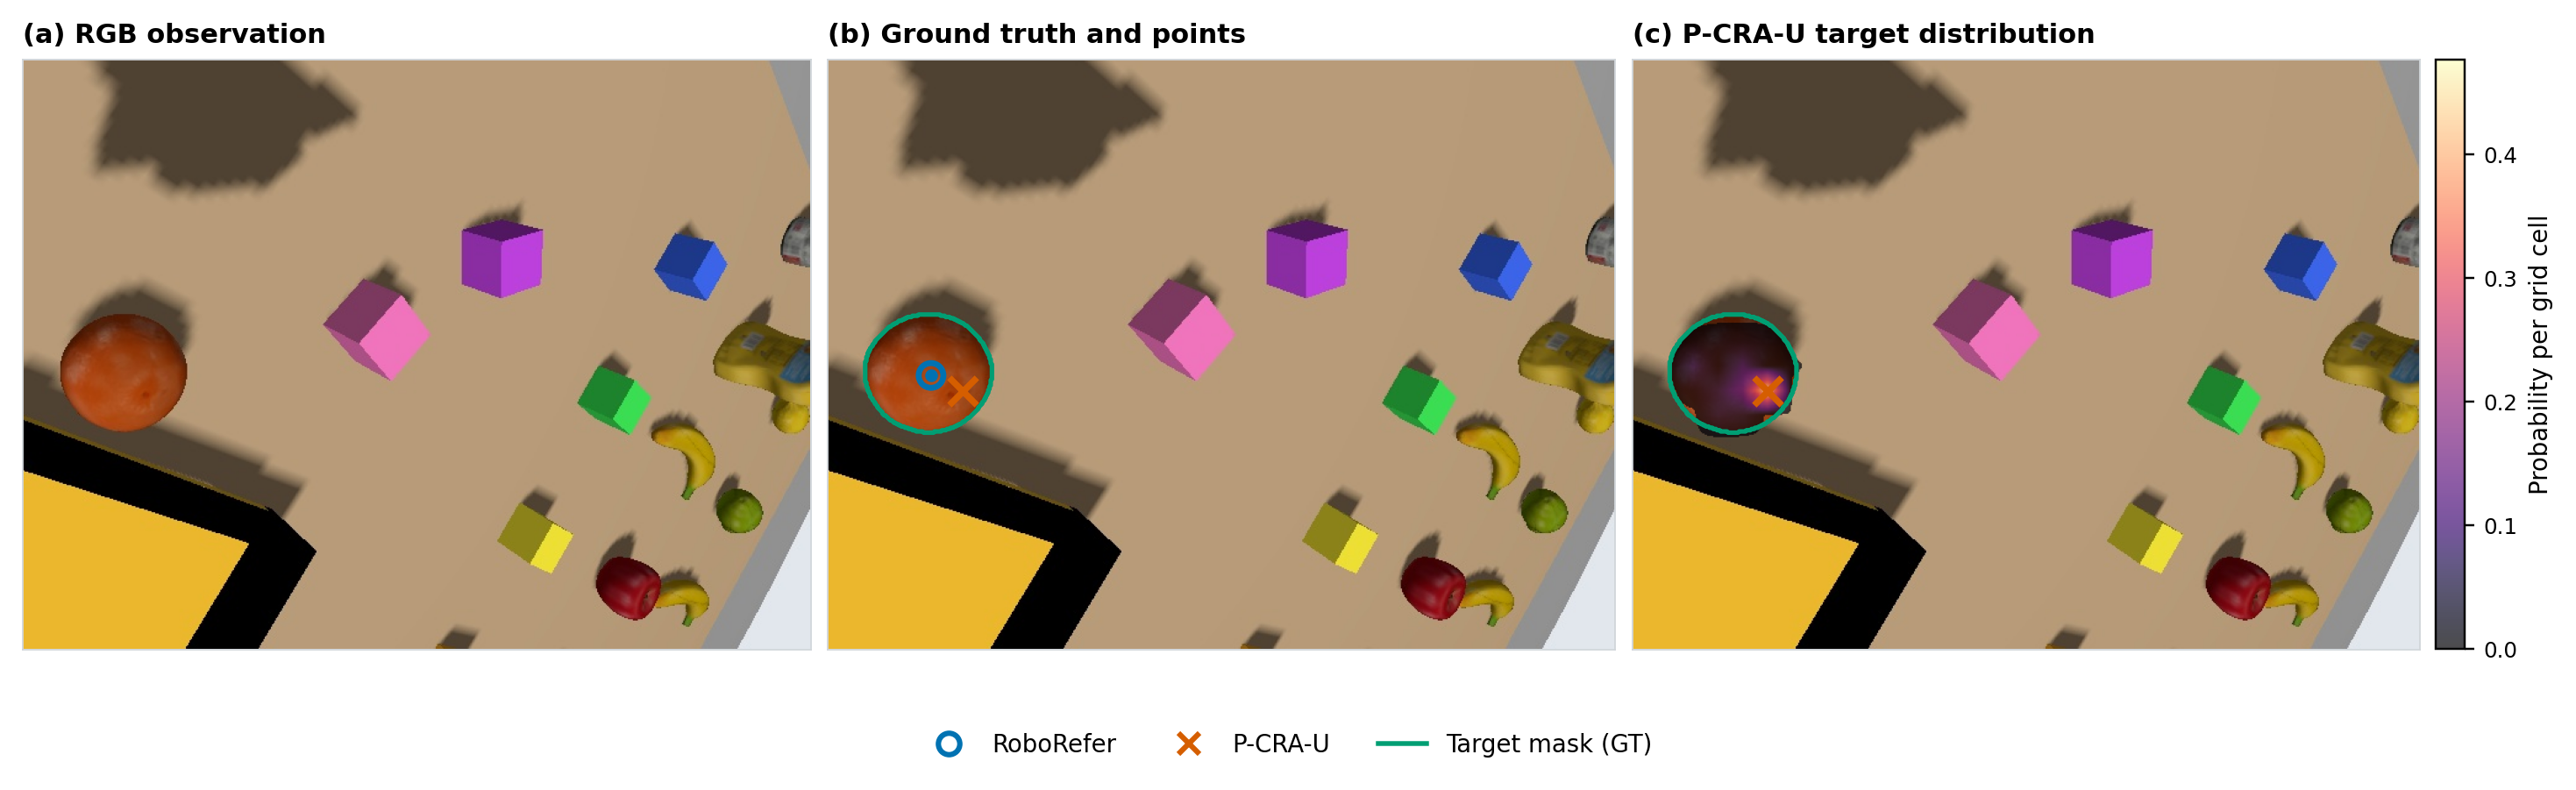
\includegraphics[width=\textwidth]{hinhanh/fig06_target_heatmap_real_rgb.png}
    \caption{Minh họa target heatmap V2 trên ảnh RGB chụp từ Gazebo.
    Điểm RoboRefer và điểm MAP của V2 được đối chiếu với vùng target.
    Heatmap được nội suy để hiển thị, không làm tăng độ phân giải dự đoán.}
    \label{fig:method-target-heatmap}
    {\footnotesize Nguồn: ảnh capture RGB và prediction thực của
    RoboRefer/V2 trong workspace; mẫu
    \texttt{v211iid\_family\_000127\_\_clean}. Mask chuẩn chỉ phục vụ đánh giá.\par}
\end{figure}

\subsection{Điểm MAP và phép ánh xạ về ảnh}

Đặt $(x^\star,y^\star)$ là tọa độ ô có xác suất lớn nhất.
Điểm pixel được đặt ở tâm ô:
\begin{equation}
\begin{split}
    u^\star&=\min\left(W-1,
    \left\lfloor\left(x^\star+\tfrac{1}{2}\right)
    \frac{W}{32}\right\rfloor\right),\\
    v^\star&=\min\left(H-1,
    \left\lfloor\left(y^\star+\tfrac{1}{2}\right)
    \frac{H}{24}\right\rfloor\right).
\end{split}
\end{equation}
Với ảnh $640\times480$, mỗi ô tương ứng $20\times20$ pixel.
Cách chọn tâm ô gây lượng tử hóa vị trí; đường bao mượt sau nội
suy không loại bỏ giới hạn này.

Điểm MAP luôn là một \emph{ứng viên} grounding. Nó chỉ trở thành
\texttt{selected\_point} nếu policy trả về \texttt{EXECUTE}.
Trong các quyết định còn lại, hệ thống có thể hiển thị ứng viên
để giải thích nhưng không cấp điểm đó như một mục tiêu chuyển động.

\subsection{Giữ nhiều mode thay vì trung bình toàn cục}

Với phân bố có nhiều vùng xác suất cao, trung bình toàn cục có thể
nằm giữa hai vật và không trúng vật nào. V2 vẫn sử dụng moment
toàn cục trong biểu diễn node, nhưng không dùng mean này làm điểm
hành động.

Để mô tả các mode, quy trình hậu xử lý tạo tập
\begin{equation}
    B=\{i:H_{t,i}\geq0.25\max_j H_{t,j}\},
\end{equation}
tìm các thành phần liên thông 8-neighbor trên $B$, tính khối lượng
xác suất mỗi thành phần rồi giữ tối đa ba thành phần lớn nhất.
Với mỗi thành phần, code tính mean để suy ra covariance cục bộ;
đầu ra lưu điểm đỉnh, khối lượng và covariance, không lưu riêng mean.
Đây là heuristic mô tả hình dạng heatmap: hai đỉnh nối bởi một dải
trên ngưỡng có thể bị gộp; số mode không phải số vật thể trong ảnh.

Hình~\ref{fig:method-multimodal} minh họa một mẫu \texttt{AMBIGUOUS}.
Các vòng đánh dấu đỉnh cục bộ trong hình phục vụ quan sát các peak;
chúng không phải định danh object và không nhất thiết trùng một-một
với cách đếm thành phần liên thông.

\begin{figure}[htbp]
    \centering
    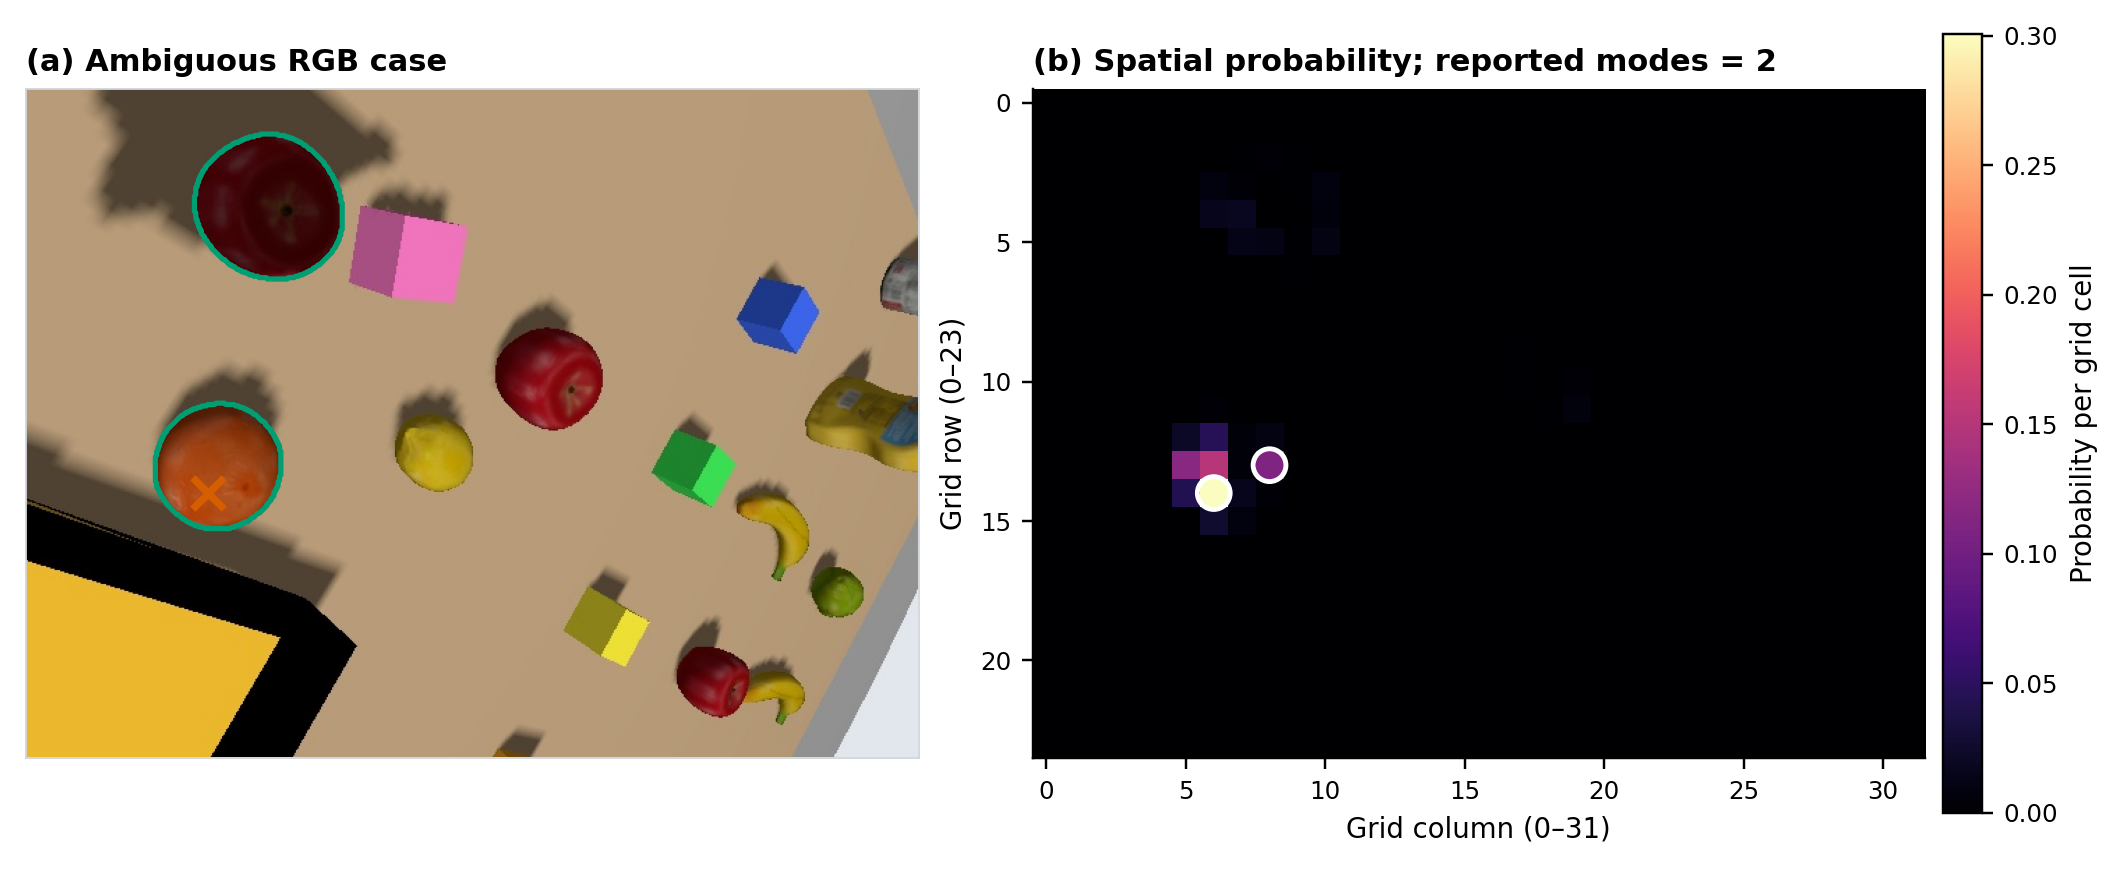
\includegraphics[width=\textwidth]{hinhanh/fig07_multimodal_spatial_distribution.png}
    \caption{Phân bố không gian đa đỉnh trên một truy vấn mơ hồ.
    Các peak tách biệt giải thích vì sao không nên lấy trung bình
    toàn cục làm điểm thao tác.}
    \label{fig:method-multimodal}
    {\footnotesize Nguồn: tác giả dựng từ RGB, heatmap và prediction
    V2 của mẫu \texttt{v211iid\_family\_000031\_\_clean} trong workspace.\par}
\end{figure}

\section{Các đặc trưng bất định không gian và đa phương thức}
\label{sec:method-uncertainty-features}

\subsection{Entropy, peak margin và mode count}

Entropy chuẩn hóa của target heatmap là
\begin{equation}
    e_{\mathrm{ent}}=
    -\frac{1}{\log N_g}
    \sum_{i=1}^{N_g}H_{t,i}\log(H_{t,i}+\epsilon).
    \label{eq:method-normalized-entropy}
\end{equation}
Giá trị gần 0 ứng với phân bố tập trung; giá trị gần 1 ứng với
phân bố gần đều. Entropy thấp không bảo đảm điểm đúng vì mô hình
có thể tự tin vào sai vùng.

Peak margin được tính bằng
\begin{equation}
    e_{\mathrm{margin}}=H_{t,(1)}-H_{t,(2)},
\end{equation}
với $H_{t,(1)}$ và $H_{t,(2)}$ là hai xác suất ô lớn nhất.
Hai ô này có thể cùng thuộc một vật, nên margin không trực tiếp
đo khoảng cách giữa hai ứng viên object.
Mode count là số thành phần được giữ bởi quy trình ở
Mục~\ref{sec:method-spatial-head}, giới hạn tối đa 3.

\subsection{Thống kê cục bộ của từng mode}

Với thành phần $\mathcal{M}_k$, đặt
\begin{equation}
    \omega_k=\sum_{i\in\mathcal{M}_k}H_{t,i},\qquad
    \widetilde{H}_{k,i}=H_{t,i}/\omega_k.
\end{equation}
Mean và covariance cục bộ là
\begin{equation}
    \mu_k=\sum_{i\in\mathcal{M}_k}\widetilde{H}_{k,i}\xi_i,\qquad
    \Sigma_k=\sum_{i\in\mathcal{M}_k}
    \widetilde{H}_{k,i}(\xi_i-\mu_k)(\xi_i-\mu_k)^{\mathsf T},
\end{equation}
trong đó $\xi_i$ là tọa độ ô. Covariance mô tả độ phân tán và được
lưu trong đầu ra hậu xử lý; mean là giá trị trung gian khi tính.
Covariance cục bộ không thuộc
vector 18 chiều của calibrator V2 và cũng chưa phải covariance
sai số đo 3D đã được kiểm chứng.

\subsection{Bất đồng với RoboRefer và tín hiệu fusion}

Nếu có điểm RoboRefer, độ bất đồng chuẩn hóa được tính bằng
\begin{equation}
    e_{RR}=
    \frac{\|p_{RR}-p_{\mathrm{PCRA}}\|_2}
    {\sqrt{W^2+H^2}}.
\end{equation}
Với ảnh hiện tại, mẫu số bằng 800 pixel.
Khi thiếu $p_{RR}$, giá trị được điền bằng 0 và một cờ missing
được đặt bằng 1. Điền 0 ở đây không có nghĩa hai mô hình đồng ý.

Các tín hiệu bổ sung gồm trung bình gate theo mọi ô và kênh,
cosine similarity và sai khác tuyệt đối trung bình giữa hai
thumbnail đặc trưng:
\begin{equation}
    e_{\mathrm{cos}}=
    \frac{r_{\mathrm{thumb}}^{\mathsf T}d_{\mathrm{thumb}}}
    {\|r_{\mathrm{thumb}}\|_2\|d_{\mathrm{thumb}}\|_2+\epsilon},
    \qquad
    e_{\mathrm{mae}}=\frac{1}{1152}
    \sum_j|r_{\mathrm{thumb},j}-d_{\mathrm{thumb},j}|.
\end{equation}
Đây là bằng chứng tương thích trong không gian embedding, không
phải phép đo độ chính xác cảm biến hay lỗi đăng ký depth.

\subsection{Điểm tổng hợp bằng chứng quan hệ}

Trên các slot có relation và anchor hoạt động từ câu lệnh,
\begin{equation}
    e_{\mathrm{rel}}=
    \frac{1}{|\mathcal{E}_{\mathrm{active}}|}
    \sum_{l\in\mathcal{E}_{\mathrm{active}}}p_l^{\mathrm{edge}}.
\end{equation}
Nếu không có cạnh hữu hiệu, implementation dùng giá trị quy ước
bằng 1. Vì vậy, điểm này cần được đọc cùng cấu trúc câu lệnh;
giá trị 1 trong truy vấn trực tiếp không chứng minh một quan hệ
đã được xác minh.

\section{Nhánh bất định theo nguồn}
\label{sec:method-source-head}

\subsection{Đặc trưng toàn cục}

Mạng kết hợp đặc trưng không gian, văn bản, quan hệ, đồ thị và
thumbnail:
\begin{equation}
\begin{split}
    h_{\mathrm{global}}=[&
    \operatorname{Mean}_{i}(F_i);
    \operatorname{Max}_{i}(F_i);
    c_q;c_r;h_Q;h_{\mathrm{thumb}}],\\
    h_{\mathrm{thumb}}={}&
    W_{\mathrm{tr}}r_{\mathrm{thumb}}+b_{\mathrm{tr}}
    +W_{\mathrm{td}}d_{\mathrm{thumb}}+b_{\mathrm{td}}.
\end{split}
\end{equation}
Vector có $6d=768$ chiều. Mean pooling mô tả bối cảnh phân bố;
max pooling giữ các đáp ứng nổi bật; $h_Q$ bổ sung bằng chứng
target--anchor liên quan trực tiếp đến truy vấn.

\subsection{Bài toán phân loại đa nhãn}

Head source có LayerNorm, lớp tuyến tính $768\rightarrow256$,
GELU, dropout và lớp tuyến tính $256\rightarrow5$:
\begin{equation}
    s_{\mathrm{src}}=
    \operatorname{Head}_{\mathrm{src}}(h_{\mathrm{global}}),
    \qquad p_k^{\mathrm{src}}=\sigma(s_k^{\mathrm{src}}).
\end{equation}
Năm nguồn là semantic, relation, spatial, depth và occlusion.
Một mẫu có thể mang nhiều nguồn cùng lúc, nên dùng sigmoid độc
lập, không dùng softmax và không yêu cầu tổng năm score bằng 1.

Semantic phản ánh bất định liên quan đến tham chiếu/ngữ nghĩa;
relation phản ánh khó khăn từ điều kiện quan hệ; spatial phản
ánh mơ hồ vị trí theo nhãn yếu đang dùng; depth phản ánh suy giảm
thông tin độ sâu; occlusion phản ánh thiếu bằng chứng do che khuất.
Các ý nghĩa này gắn với cách tạo supervision của dataset, không
phải phân rã nhân quả hoàn chỉnh của mọi lỗi grounding.

\subsection{Nhãn yếu và cách diễn giải score}

Trong V2, source spatial được gán từ trạng thái \texttt{AMBIGUOUS}
và có trọng số loss bằng 0.5. Do đó, đây là nhãn yếu về mơ hồ,
không phải nhãn đo trực tiếp độ bất định vật lý.
Các source còn lại dựa trên supervision của biến thể dữ liệu.
Nhánh counterfactual ranking bổ sung tương phản giữa biến thể
sạch và biến thể gây nhiễu, như trình bày ở
Mục~\ref{sec:method-loss}.

Snapshot calibrator V2 không có bộ ngưỡng riêng đã tối ưu cho từng
source; ngưỡng báo nguồn hoạt động mặc định là 0.5.
Các score source chưa được hiệu chuẩn riêng thành xác suất lỗi
theo nguồn. Chúng tham gia vector bằng chứng để calibrator ước
lượng rủi ro grounding chung.

\begin{figure}[htbp]
    \centering
    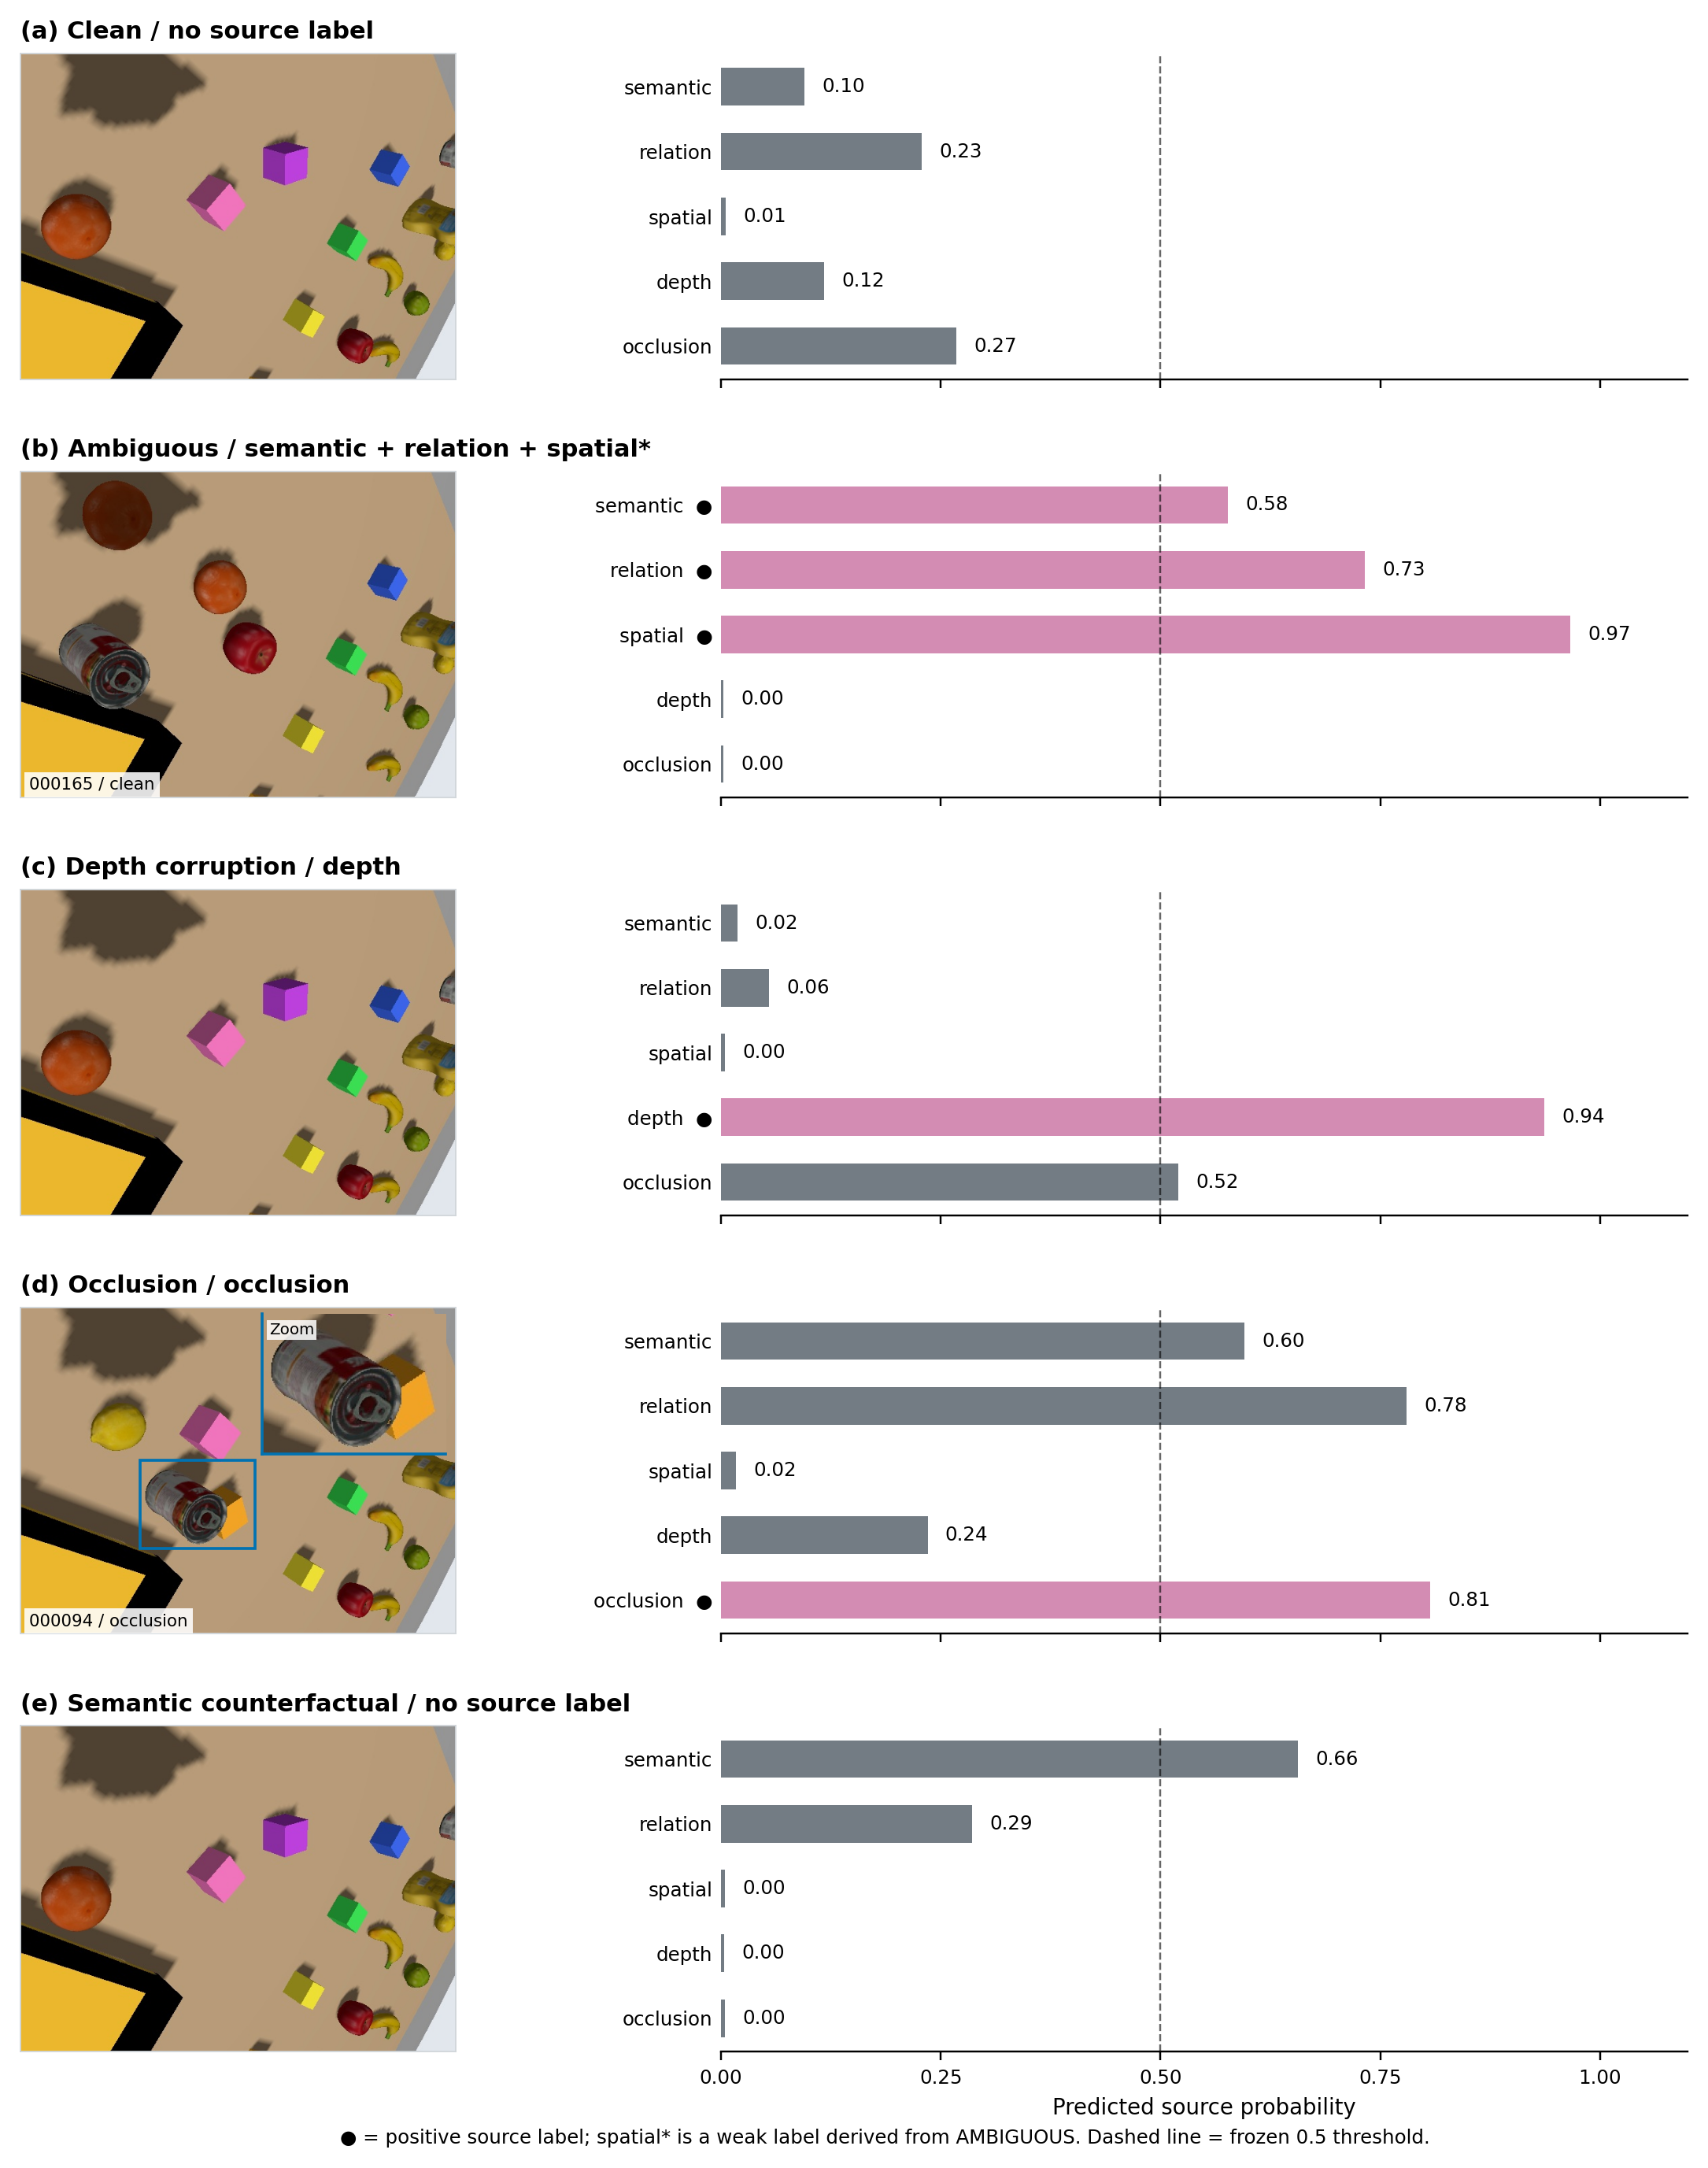
\includegraphics[width=\textwidth]{hinhanh/fig08_source_uncertainty_cases.png}
    \caption{Minh họa năm score source uncertainty trên các quan sát
    và biến thể thực. Nhãn chuẩn được đối chiếu để giải thích đầu ra;
    hình bao gồm cả trường hợp báo nguồn chưa đúng.}
    \label{fig:method-source-cases}
    {\footnotesize Nguồn: tác giả dựng từ ảnh capture, supervision
    và prediction V2 đã lưu trong workspace; không tạo ảnh minh họa bằng AI.\par}
\end{figure}

\section{Nhánh đánh giá khả năng trả lời}
\label{sec:method-answer-head}

\subsection{Bốn trạng thái answerability}

Head answerability dùng cùng $h_{\mathrm{global}}$ nhưng có tham số
riêng với source head. Đầu ra là bốn logits:
\begin{equation}
    s_{\mathrm{ans}}=
    \operatorname{Head}_{\mathrm{ans}}(h_{\mathrm{global}}),
    \qquad p_c^{\mathrm{ans}}=
    \frac{\exp(s_c^{\mathrm{ans}})}
    {\sum_{j=1}^{4}\exp(s_j^{\mathrm{ans}})}.
\end{equation}
Bốn lớp loại trừ nhau theo ontology:
\begin{description}
    \item[\texttt{FOUND}:] có một target hợp lệ với bằng chứng đủ
    theo câu lệnh và quy tắc gán nhãn.
    \item[\texttt{AMBIGUOUS}:] có nhiều ứng viên hợp lệ mà câu lệnh
    chưa phân biệt được.
    \item[\texttt{ABSENT}:] không có target thỏa yêu cầu trong
    phạm vi cảnh được gán nhãn.
    \item[\texttt{INSUFFICIENT\_EVIDENCE}:] quan sát hiện tại chưa
    đủ để kết luận, chẳng hạn vì che khuất hoặc dữ liệu cảm biến.
\end{description}
Trạng thái dự đoán là $\widehat{c}=\arg\max_c p_c^{\mathrm{ans}}$.
Phân biệt \texttt{ABSENT} và \texttt{INSUFFICIENT\_EVIDENCE} quan
trọng vì một trường hợp cần dừng, còn trường hợp kia có thể cần
quan sát lại.

\subsection{Adapter answerability trên evidence đóng băng}
\label{sec:method-answer-adapter}

Head gốc ở trên tạo $s_{\mathrm{ans}}^{V2}$. Phiên bản được chọn
bổ sung một mạng phần dư, chỉ dùng đặc trưng dự đoán và quan sát:
\begin{equation}
    s_{\mathrm{ans}}=s_{\mathrm{ans}}^{V2}+\Delta_\psi(z),
    \qquad p^{\mathrm{ans}}=\operatorname{softmax}(s_{\mathrm{ans}}).
    \label{eq:method-answer-adapter}
\end{equation}
Vector $z$ có 2222 chiều: 26 evidence tóm tắt và 2196 chiều chi tiết
gồm embedding toàn cục, query/node target--relation--anchor và spatial
moments. Evidence tóm tắt gồm kích hoạt target/interior/anchor,
peak, entropy, top-5/top-10 mass, độ lệch đỉnh target--interior,
edge, gate, tương thích RGB-D, năm source và bốn xác suất V2 gốc.
Chúng không chứa mask chuẩn, nhãn answerability, family ID hoặc variant.
Slot không hoạt động được xử lý theo mask truy vấn.

Mean/scale chỉ fit trên train; evidence chuẩn hóa được chặn vào
$[-5,5]$. Mạng $2222\rightarrow64\rightarrow4$ dùng GELU và dropout
0.3; lớp cuối khởi tạo bằng 0 để ban đầu giữ đúng logits V2.
RoboRefer và toàn bộ sidecar V2 được đóng băng trong bước này.
Adapter thay phân loại khả năng trả lời, không thay MAP hoặc mask dự đoán.

\subsection{Tách answerability khỏi độ sắc của heatmap}

Độ sắc của heatmap chỉ mô tả cách mô hình phân bổ xác suất vị trí.
Answerability còn sử dụng ngữ cảnh câu lệnh và embedding đồ thị,
nên có thể từ chối một heatmap rất tập trung nếu bằng chứng chỉ
ra vật đích không tồn tại. Ngược lại, một heatmap có nhiều đỉnh
không tự động đồng nghĩa \texttt{AMBIGUOUS}: một số đỉnh có thể
không thỏa câu lệnh.

Hai head answerability và source cùng được huấn luyện với các
head không gian. Đây là học đa nhiệm trên cùng biểu diễn, không
phải các module kiểm tra độc lập hoàn toàn.
Các sai số tương quan giữa chúng là lý do cần bộ hiệu chuẩn
ở giai đoạn tiếp theo.

\section{Định vị 3D từ metric depth}
\label{sec:method-3d}

\subsection{Suy ngược điểm trong hệ tọa độ camera}

Khi đã có ứng viên pixel $(u^\star,v^\star)$ và metric depth hợp lệ
$z^\star$, với camera pinhole đã đăng ký ảnh:
\begin{equation}
    P_{\mathrm{camera}}=
    z^\star K^{-1}
    \begin{bmatrix}u^\star\\v^\star\\1\end{bmatrix},
    \qquad
    K=
    \begin{bmatrix}
        f_x&0&c_x\\
        0&f_y&c_y\\
        0&0&1
    \end{bmatrix}.
    \label{eq:method-backprojection}
\end{equation}
Depth dùng ở đây phải phù hợp quy ước $z$ theo trục quang học của
camera, không phải một ảnh relative depth hoặc khoảng cách tia
chưa chuyển đổi. Nếu ảnh có méo chưa được hiệu chỉnh, cần xử lý
méo trước khi áp dụng mô hình này \cite{opencvCameraModel}.

Không nên lấy depth ở một pixel nếu nó không hữu hạn, thuộc nền
bàn hoặc nằm trên biên che khuất. Có thể dùng thống kê lân cận
để giảm nhiễu, nhưng phải giữ điều kiện vùng đó thuộc vật đích;
không lấy trung bình xuyên qua hai bề mặt có độ sâu khác nhau.

\subsection{Chuyển sang hệ tọa độ robot}

Với phép biến đổi đồng nhất từ camera sang base:
\begin{equation}
    \begin{bmatrix}P_{\mathrm{base}}\\1\end{bmatrix}
    =
    T_{\mathrm{base}\leftarrow\mathrm{camera}}
    \begin{bmatrix}P_{\mathrm{camera}}\\1\end{bmatrix}.
\end{equation}
Khi dùng camera cổ tay, TF phụ thuộc cấu hình joint và thời điểm
capture. Khi dùng camera ngoài, vẫn cần xác minh extrinsic và
quy ước optical frame. Việc trộn hệ tọa độ camera optical với
hệ tọa độ link camera có thể làm sai hướng trục dù tọa độ pixel
grounding đúng \cite{foote2010rep103}.

\subsection{Phạm vi của đầu ra hình học}

Các công thức trên mô tả giao diện cần thiết cho thao tác robot.
Policy V2 hiện không nhận $K$, $T$ hay một biến
\texttt{geometry\_pass}; do đó không được diễn giải
\texttt{EXECUTE} thành đã đạt mọi điều kiện hình học.

Trước khi nối MoveIt cần tối thiểu kiểm tra đồng bộ RGB-D/TF,
depth hợp lệ, vật đích độc lập và độ ổn định điểm qua nhiều
khung hình. Sau đó mới đánh giá khả năng tiếp cận, va chạm,
tư thế gắp và trạng thái gripper. Các phép kiểm tra này không
được sử dụng để âm thầm thay điểm prediction bằng tọa độ
ground-truth của scene.
Trong phạm vi thực nghiệm grounding của đồ án, đầu ra 3D là
thành phần thứ cấp; chưa có cơ sở để công bố covariance 3D
đã hiệu chuẩn hay tỉ lệ pick-and-place thành công chỉ từ chỉ
số point-in-target trên ảnh.

\section{Bộ hiệu chuẩn rủi ro độc lập}
\label{sec:method-calibrator}

\subsection{Biến cố lỗi cần dự đoán}

Bộ hiệu chuẩn không học nhãn “heatmap sắc hay mờ”, mà học biến cố
lỗi grounding theo định nghĩa đánh giá:
\begin{equation}
    y_{\mathrm{err}}=
    \mathbf{1}\left[
    y_{\mathrm{ans}}\neq\texttt{FOUND}
    \ \lor\ p_{\mathrm{PCRA}}\notin M_t
    \right],
    \label{eq:method-error-event}
\end{equation}
với $M_t$ là mask target chuẩn ở độ phân giải ảnh.
Như vậy, một điểm nằm trong vùng ứng viên của câu lệnh mơ hồ vẫn
không được coi là grounding có thể chấp nhận để thực thi.
Nhãn lỗi này chỉ dùng khi fit và đánh giá calibrator;
ở suy luận, hệ thống không truy cập $M_t$ hay $y_{\mathrm{ans}}$.

Rủi ro cần ước lượng là
\begin{equation}
    r_{\mathrm{ground}}(x)
    \approx \Pr(y_{\mathrm{err}}=1\mid e(x)).
\end{equation}
Đây là rủi ro của grounding trong ảnh theo ontology đã chọn,
không phải xác suất va chạm hay xác suất gắp thất bại của robot.

\subsection{Vector bằng chứng của V2 và phiên bản Adapter}

V2 lịch sử dùng vector 18 chiều, khóa theo thứ tự:
\begin{equation}
\begin{split}
    e=[&
    e_{\mathrm{ent}},e_{\mathrm{margin}},N_{\mathrm{mode}},\\
    &p_{\mathrm{FOUND}}^{\mathrm{ans}},
    p_{\mathrm{AMBIGUOUS}}^{\mathrm{ans}},
    p_{\mathrm{ABSENT}}^{\mathrm{ans}},
    p_{\mathrm{INSUFFICIENT\_EVIDENCE}}^{\mathrm{ans}},\\
    &p_{\mathrm{semantic}}^{\mathrm{src}},
    p_{\mathrm{relation}}^{\mathrm{src}},
    p_{\mathrm{spatial}}^{\mathrm{src}},
    p_{\mathrm{depth}}^{\mathrm{src}},
    p_{\mathrm{occlusion}}^{\mathrm{src}},\\
    &e_{\mathrm{rel}},\overline{g},
    e_{\mathrm{cos}},e_{\mathrm{mae}},e_{RR},m_{RR}].
\end{split}
\end{equation}
$m_{RR}$ là cờ thiếu điểm RoboRefer. Tất cả bằng chứng trên được
tính từ prediction và dữ liệu quan sát. Vector này không
chứa metric geometry, TF, local covariance, tỉ lệ pixel depth
hợp lệ hay nhãn chất lượng cảm biến trực tiếp.

Trong artifact V2 lịch sử, hai hệ số của $e_{RR}$ và
$m_{RR}$ đều bằng 0. Dữ liệu fit có điểm RoboRefer bị thiếu ở
hai chiều này, nên calibrator chưa học được tác dụng của độ
bất đồng. Dù giao diện hỗ trợ tính $e_{RR}$, không được quy
cải thiện calibration của V2 cho tín hiệu chưa có ảnh hưởng
trong artifact đã fit.

P-CRA-U hiện tại giữ 18 chiều này nhưng dùng xác suất answerability
sau Adapter, rồi nối thêm 15 evidence: max/mean sigmoid target,
peak và top-5/top-10 mass, max/mean sigmoid interior,
khoảng cách đỉnh target--interior, mean/min cực đại anchor,
min edge và bốn xác suất answerability V2 trước Adapter.
Tổng cộng $e^{\mathrm{Adapter}}\in\mathbb{R}^{33}$.
Vector 33 chiều của calibrator khác vector 2222 chiều đầu vào Adapter.
Nó vẫn chưa chứa metric geometry/TF; hai hệ số disagreement/missing
cũng bằng 0 trong calibrator được chọn.

\subsection{Chuẩn hóa và logistic calibration}

Sau khi đóng băng checkpoint sidecar, mỗi chiều evidence được
chuẩn hóa bằng thống kê của tập calibration:
\begin{equation}
    \widetilde{e}_j=\frac{e_j-\mu_j}{\sigma_j}.
\end{equation}
Nếu $\sigma_j<10^{-8}$, scale được đặt bằng 1.
Bộ hiệu chuẩn là hồi quy logistic có regularization:
\begin{equation}
    C_\phi(e)=\sigma(w^{\mathsf T}\widetilde{e}+b),
    \label{eq:method-logistic}
\end{equation}
\begin{equation}
    \mathcal{L}_{\mathrm{cal}}=
    -\frac{1}{n}\sum_{i=1}^{n}
    \left[y_i\log r_i+(1-y_i)\log(1-r_i)\right]
    +\frac{\lambda_{\mathrm{cal}}}{2}\|w\|_2^2.
\end{equation}
V2 dùng $\lambda_{\mathrm{cal}}=10^{-3}$, Adapter dùng $10^{-2}$. Intercept $b$ không bị regularize. Implementation dùng cập nhật
Newton với ổn định số cho Hessian và tối đa 100 vòng lặp.
Cách dùng một mô hình nhỏ sau mạng chính phù hợp với nguyên tắc
hiệu chuẩn hậu huấn luyện \cite{niculescu2005probabilities,guo2017calibration};
tuy nhiên, đây là logistic trên nhiều evidence, không phải
temperature scaling một scalar logit.

\subsection{Cross-fitting theo family}

Tập calibration hiện tại có 200 family, mỗi family có năm variant.
Các variant cùng family không được tách ra các fold khác nhau.
Ở V2 lịch sử, fold được xác định tái lập bằng hash family ID:
\begin{equation}
    f(\mathrm{family})=
    \operatorname{hash}_{64}(\mathrm{family})\bmod5.
\end{equation}
Ở Adapter, các family được sắp theo SHA-256 của ID rồi phân luân phiên vào năm fold; mỗi fold giữ 40 family. Ở mỗi fold, mean, scale và logistic được fit trên bốn fold còn
lại rồi dự đoán fold giữ lại. Ghép các prediction này tạo risk
cross-fit cho toàn bộ calibration.

Sau cross-fitting, calibrator cuối cùng được fit lại trên toàn
bộ tập calibration. Các tham số chuẩn hóa, hệ số logistic,
ngưỡng risk và khối lượng vùng tin cậy được lưu thành artifact.
Đánh giá lại Test-IID chỉ sử dụng artifact đã đóng băng; không fit tham số bằng test. Bộ IID cũ đã được phân tích, nên không được coi là tập xác nhận mới chưa quan sát.

\subsection{Chọn ngưỡng rủi ro của V2 lịch sử}

Với ngưỡng ứng viên $\tau$, tập chấp nhận theo risk là
\begin{equation}
    \mathcal{A}_{\tau}=
    \{i:r_i^{\mathrm{crossfit}}\leq\tau\},\qquad
    \widehat{R}_{\tau}=
    \frac{\sum_{i\in\mathcal{A}_{\tau}}y_i}
    {|\mathcal{A}_{\tau}|}.
\end{equation}
Code duyệt các giá trị risk phân biệt và chọn ngưỡng lớn nhất
thỏa hai điều kiện: tập chấp nhận có ít nhất 60 family và
cận trên Wilson 95\% của tỉ lệ lỗi không vượt mục tiêu 0.05.
Với $n_\tau$ mẫu chấp nhận, $\widehat{p}=\widehat{R}_{\tau}$
và $z=1.96$, cận trên được tính:
\begin{equation}
    U_{\mathrm{Wilson}}=
    \frac{\widehat{p}+\frac{z^2}{2n_\tau}
    +z\sqrt{\frac{\widehat{p}(1-\widehat{p})}{n_\tau}
    +\frac{z^2}{4n_\tau^2}}}
    {1+\frac{z^2}{n_\tau}}.
\end{equation}
Nếu không có ngưỡng đạt điều kiện, threshold được lưu là
không xác định và nhánh risk không cho phép \texttt{EXECUTE}.
Ngưỡng trong artifact V2 lịch sử là
$\tau=0.09370088241237143$.

Cần phân biệt phép chọn ngưỡng này với một bảo đảm rủi ro hữu
hạn mẫu ở cấp family. Cận Wilson hiện được tính trên số
\emph{variant}, trong khi các variant cùng family phụ thuộc;
đồng thời code duyệt nhiều ngưỡng mà không điều chỉnh cho việc
lựa chọn nhiều lần. Điều kiện tối thiểu 60 family không tự khắc
phục hai vấn đề đó. Vì vậy, đây là quy tắc chọn ngưỡng thực nghiệm,
không phải chứng minh rằng risk tương lai chắc chắn dưới 5\%.
Khoảng tin cậy của kết quả Test-IID phải được báo cáo bằng bootstrap
theo family ở chương đánh giá.

Tập chấp nhận risk khi chọn $\tau$ cũng chưa áp điều kiện
answerability của policy. Ở quyết định cuối, \texttt{FOUND}
được yêu cầu thêm. Vì vậy, risk-only coverage và tỉ lệ
\texttt{EXECUTE} không nhất thiết bằng nhau.

\subsection{Ngưỡng của P-CRA-U có Adapter}
\label{sec:method-adapter-threshold}

Phiên bản được chọn dùng policy \texttt{hard\_found}, nên tập chọn ngưỡng là
\begin{equation}
    \mathcal{A}^{\mathrm{Adapter}}_\tau=
    \{i:\arg\max p_i^{\mathrm{ans}}=\mathrm{FOUND},\ 
      r_i^{\mathrm{crossfit}}\leq\tau\}.
\end{equation}
Code chọn ngưỡng có coverage lớn nhất thỏa tối thiểu 60 family và
cận Wilson 95\% không vượt ngân sách 7.5\% trên calibration ngoài fold.
Hai ứng viên logistic18 ($\lambda=0.001$) và logistic33
($\lambda=0.01$) được so theo Brier cross-fit; logistic33 được chọn.
Artifact khóa $\tau=0.2611932834526145$, khác ngân sách lỗi 0.075:
ngưỡng áp cho risk của từng quan sát, ngân sách áp cho tỉ lệ lỗi
trong tập chấp nhận. Calibration ngoài fold nhận 346 mẫu với 16 lỗi,
selective risk 4.62\% và cận Wilson 7.38\%.

Runtime dùng calibrator fit lại toàn calibration, không dùng mô hình
ngoài fold. Cùng ngưỡng, phép chấm lại trên chính calibration sau fit
nhận 351 mẫu với 14 lỗi; đây là resubstitution, không phải audit độc lập.
Chuyển từ cross-fit sang full-fit và chọn nhiều cấu hình/ngưỡng còn
giới hạn độ tin cậy. Test-IID cũ có lỗi 9.42\%, vượt ngân sách 7.5\%;
không diễn giải profile này là bảo đảm lỗi tương lai dưới 7.5\%.
Các giới hạn phụ thuộc family và chọn nhiều ngưỡng vẫn áp dụng.

\begin{figure}[htbp]
    \centering
    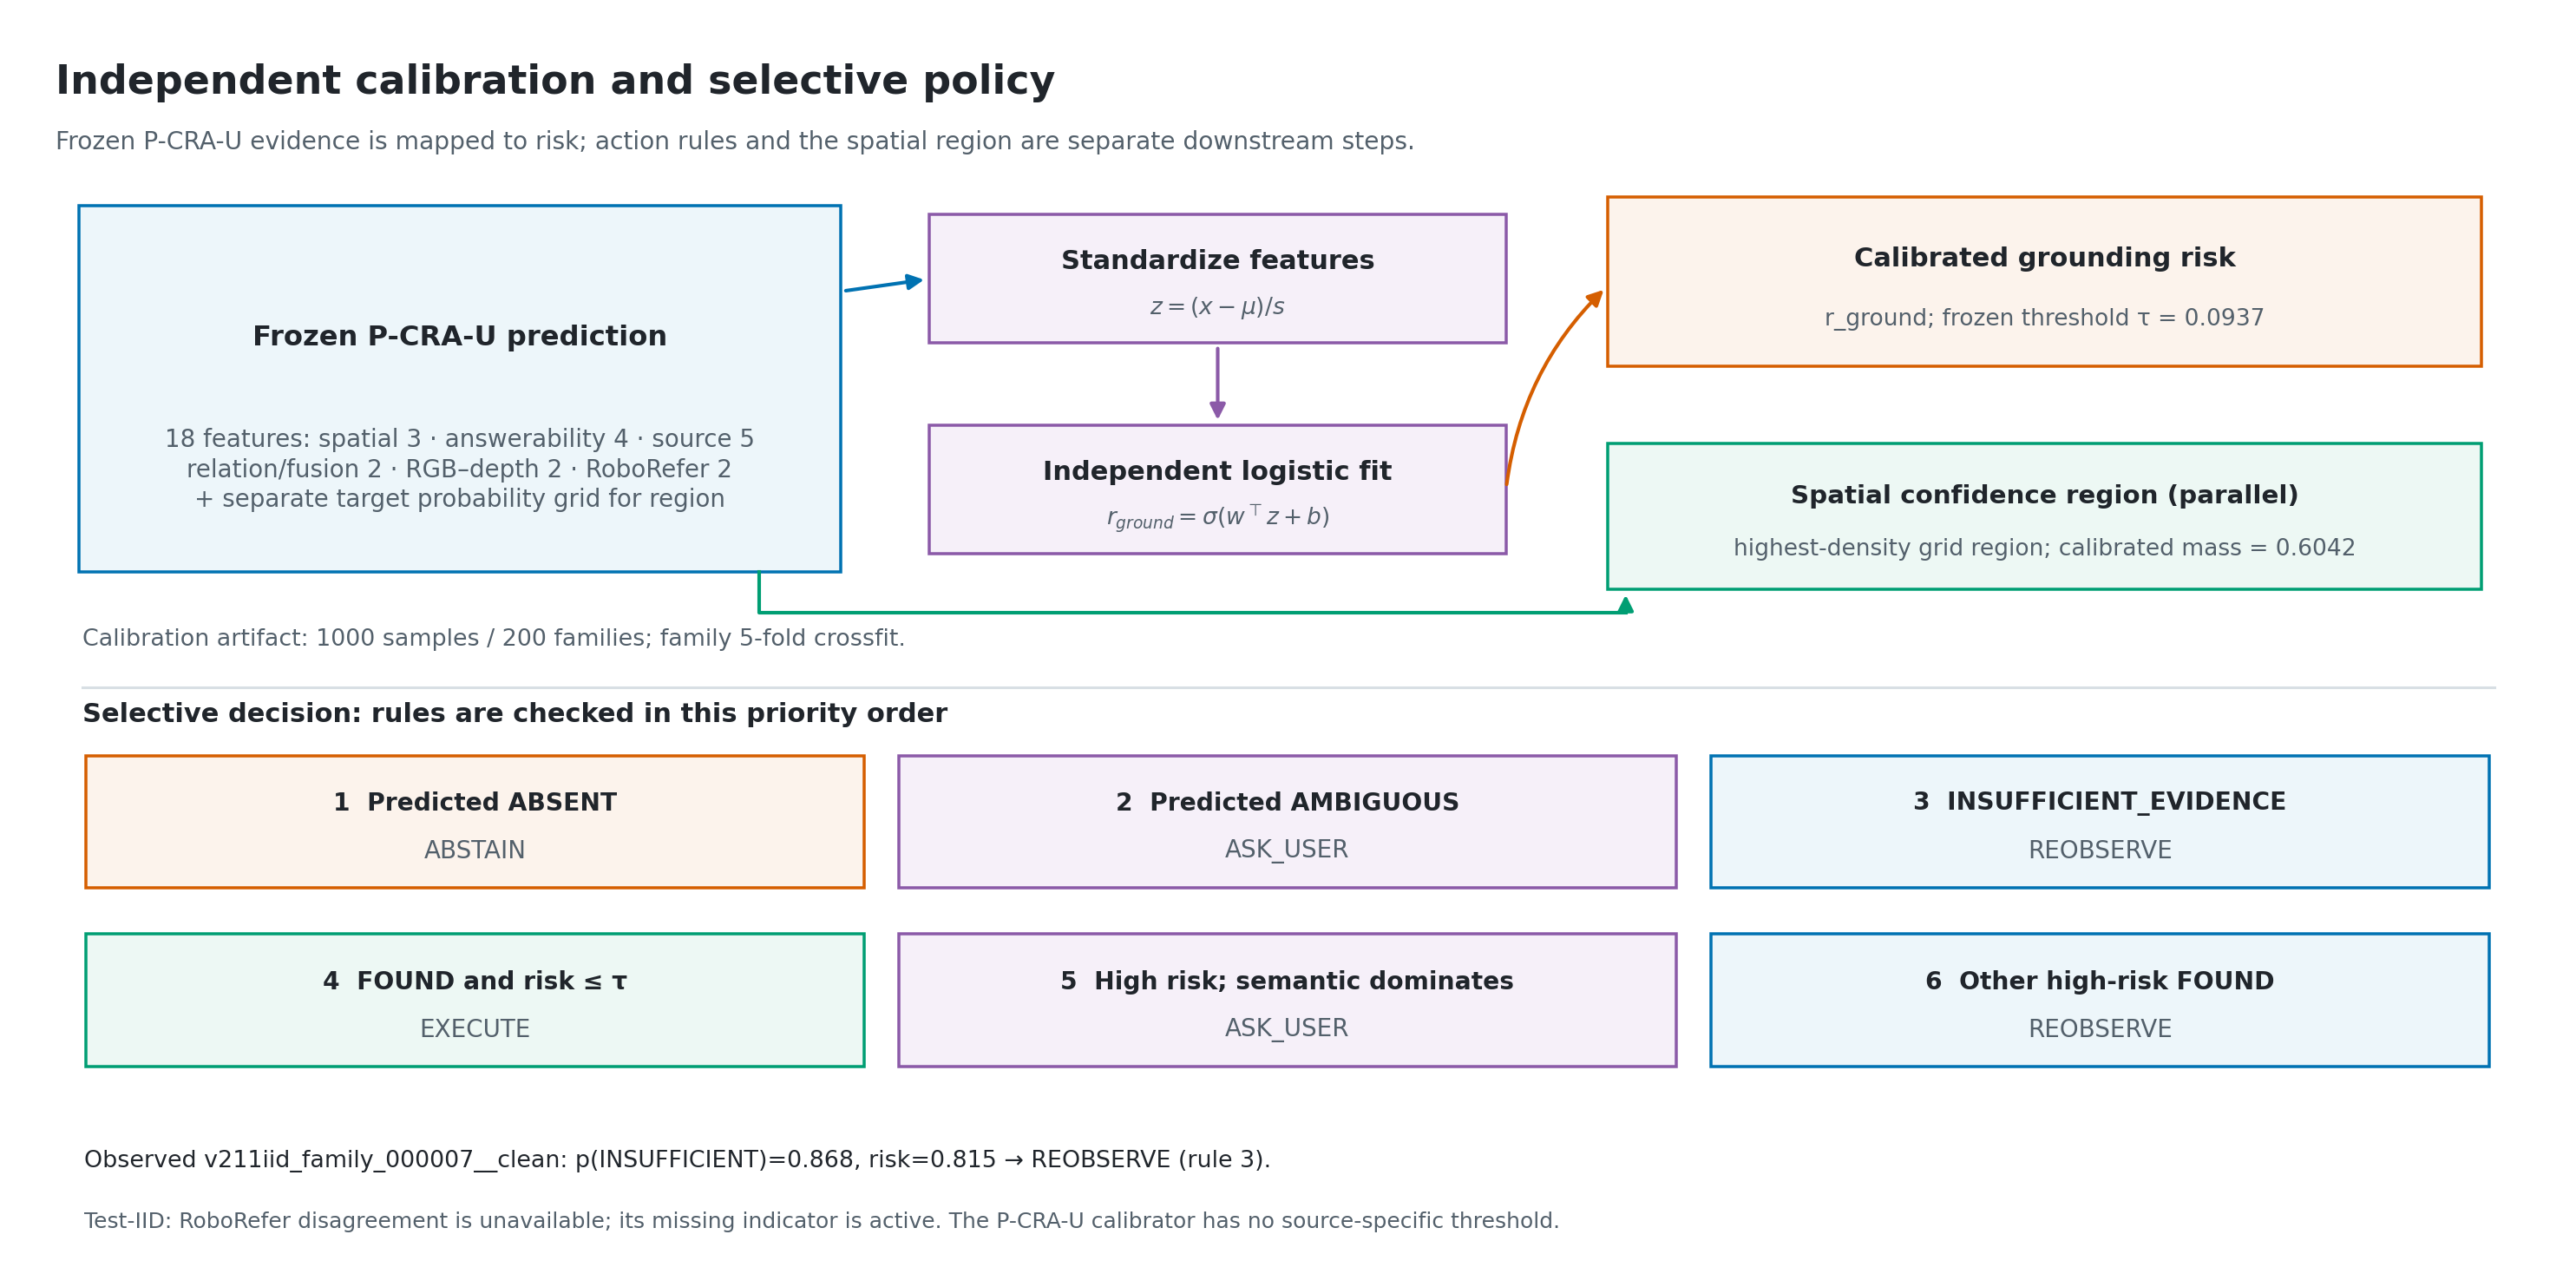
\includegraphics[width=\textwidth]{hinhanh/fig09_independent_calibrator_v2.png}
    \caption{Bộ hiệu chuẩn độc lập: evidence quan sát được, chuẩn hóa,
    logistic risk và giao diện với policy/vùng tin cậy.
    Các giá trị ngưỡng trong hình lấy từ artifact V2 đã đóng băng.}
    \label{fig:method-calibrator}
    {\footnotesize Nguồn: tác giả dựng từ code calibration/policy,
    tệp \texttt{calibrator.json} V2 và prediction thực trong workspace.\par}
\end{figure}

\section{Vùng tin cậy không gian}
\label{sec:method-confidence-region}

\subsection{Vùng highest-density trên lưới}

Ngoài điểm MAP, hệ thống có thể trả về một tập ô có tổng xác suất
đạt khối lượng $m$. Sắp xếp các ô theo xác suất giảm dần:
\begin{equation}
    H_{t,(1)}\geq H_{t,(2)}\geq\cdots\geq H_{t,(N_g)}.
\end{equation}
Đặt
\begin{equation}
    k(m)=\min\left\{k:\sum_{j=1}^{k}H_{t,(j)}\geq m\right\},
    \qquad C(m)=\{(1),\ldots,(k(m))\}.
    \label{eq:method-hd-region}
\end{equation}
Tập ô này có thể rời nhau nếu phân bố đa mode. Vì vậy,
bounding box bao vùng chỉ là thông tin tóm tắt; nó không thay
thế tập ô được chọn khi đánh giá region.
Do lưới rời rạc, khối lượng thực tế thường lớn hơn hoặc bằng $m$.

\subsection{Score calibration và phân vị hữu hạn mẫu}

Trên mỗi mẫu calibration có target, mask chuẩn được đưa về lưới.
Theo thứ tự xác suất giảm dần, tìm ô đầu tiên có giao với target
và lấy tổng xác suất tích lũy đến ô đó làm score $S_i$.
Các score được sắp xếp tăng dần. Với mức $\alpha$, khối lượng
dùng khi suy luận là
\begin{equation}
    m_\alpha=S_{(k_\alpha)},\qquad
    k_\alpha=
    \min\left(n_t,
    \left\lceil(n_t+1)(1-\alpha)\right\rceil\right),
\end{equation}
trong đó $n_t$ là số mẫu calibration có target.
V2 dùng $\alpha=0.1$, $n_t=835$, nên chọn hạng 753 và lưu
$m_\alpha=0.6041831970214844$.

Evaluator báo score coverage theo $S_i\leq m_\alpha$. Policy dựng
$C(m_\alpha)$ bằng cách nhận cả ô vượt biên để đạt khối lượng yêu cầu;
kiểm tra $C(m_\alpha)\cap M_i\neq\varnothing$ là direct-intersection
coverage. Hai event không đồng nhất trên lưới rời rạc, như đã định nghĩa
ở Chương~2 và được đối chiếu ở Chương~5. Cả hai đều chỉ hướng tới việc
vùng chạm target, không phải chứa toàn bộ vật, tâm vật hoặc điểm gắp hợp lệ.

\subsection{Giới hạn diễn giải conformal}

Quy tắc phân vị có liên hệ với split conformal prediction
\cite{angelopoulos2021conformal,lei2018distributionfree}.
Tuy nhiên, bảo đảm conformal tiêu chuẩn cần các đơn vị
calibration và test thỏa điều kiện exchangeability phù hợp.
Artifact hiện tại lấy score ở cấp variant, không phải một
score tổng hợp độc lập cho từng family.

Do vậy, đồ án gọi đây là vùng highest-density được hiệu chỉnh
bằng phân vị theo quy trình conformal, nhưng không khẳng định
bảo đảm distribution-free 90\% ở cấp family. Coverage danh
nghĩa và coverage Test-IID thực tế phải được báo cáo tách biệt.
Diện tích vùng cũng cần được báo cáo vì một vùng gần toàn ảnh
có thể giao target thường xuyên nhưng ít hữu ích cho định vị.

Vùng tin cậy được tạo sau prediction nếu artifact có khối
lượng hợp lệ, kể cả với quyết định không thực thi. Vùng này
là đầu ra giải thích/đánh giá, chưa phải vùng an toàn va chạm
của robot và không tự mở cổng hành động.

\begin{figure}[htbp]
    \centering
    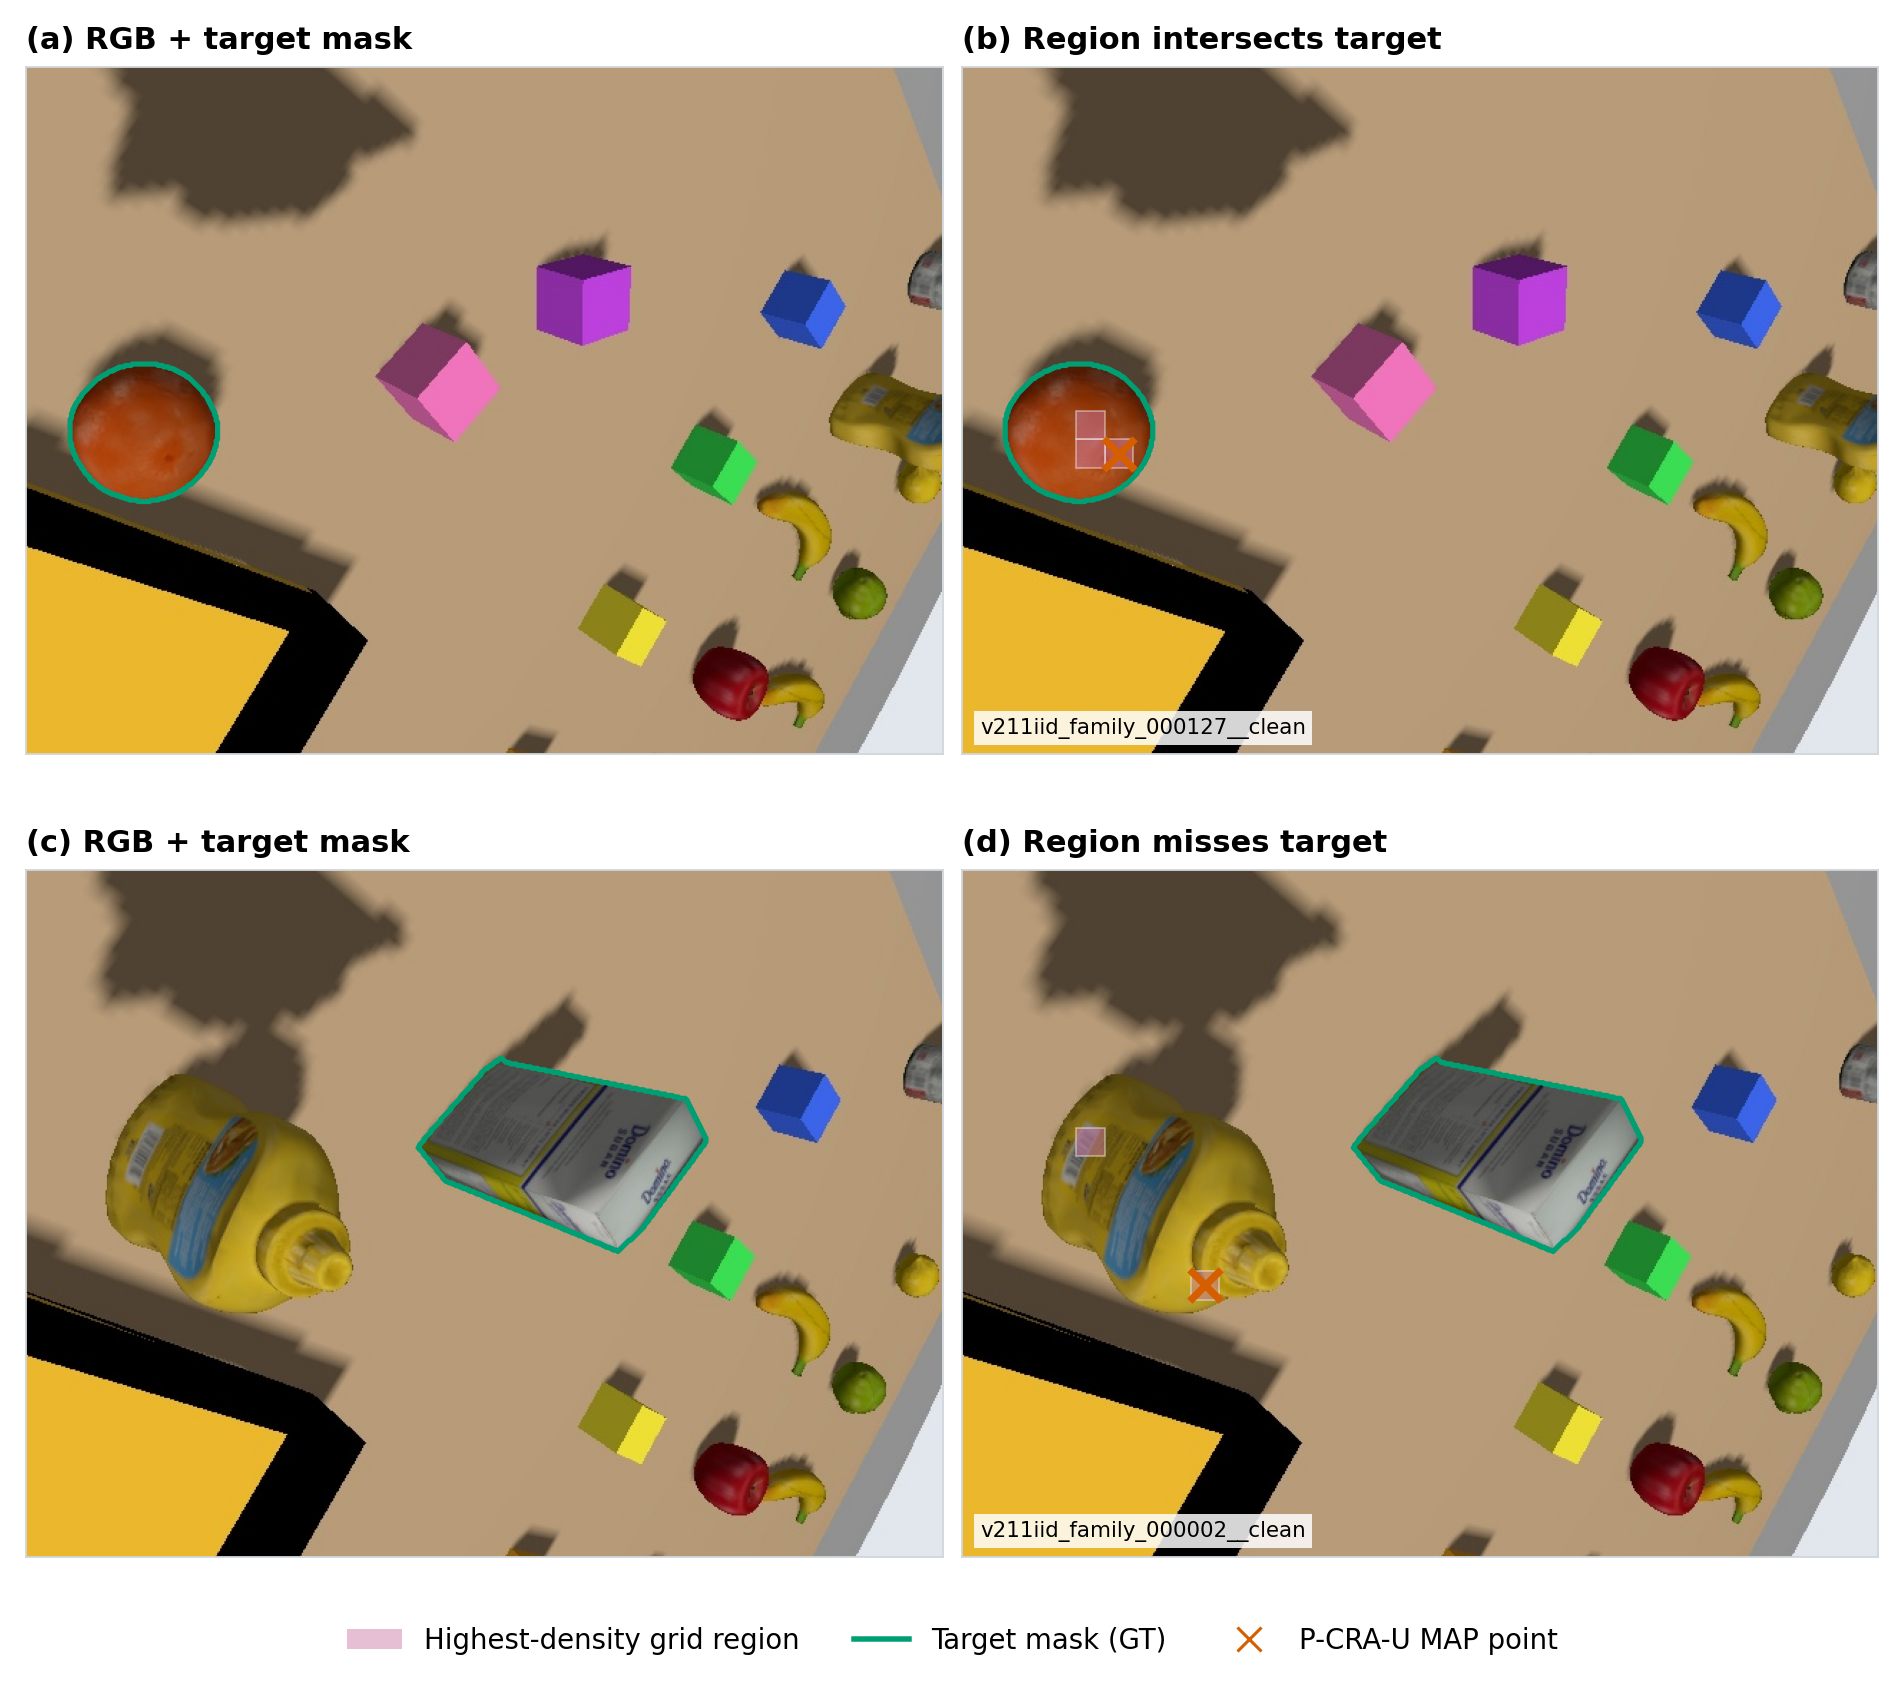
\includegraphics[width=\textwidth]{hinhanh/fig12_confidence_region_true_rgb.png}
    \caption{Vùng highest-density trên ảnh RGB thực của bộ mô phỏng:
    một trường hợp vùng giao target và một trường hợp vùng trượt target.
    Các ô được chọn lấy trực tiếp từ quyết định đã lưu, không vẽ
    ellipse thay thế cho region của mô hình.}
    \label{fig:method-confidence-region}
    {\footnotesize Nguồn: tác giả dựng từ RGB, mask đánh giá và
    decision V2 của các mẫu Test-IID trong workspace.\par}
\end{figure}

\section{Hàm mất mát và quy trình tối ưu}
\label{sec:method-loss}

\subsection{Supervision không gian và mask tính loss}

Mask target, interior và anchor ở độ phân giải ảnh được đưa về
lưới $24\times32$ bằng nội suy diện tích. Giá trị mask nhỏ
$M_i\in[0,1]$ biểu diễn tỉ lệ chiếm ô, không bắt buộc nhị phân.
Mỗi loại bản đồ có một mask validity riêng. Loss chỉ được
tính với bản đồ có vùng chuẩn không rỗng; nếu không có bản đồ
hợp lệ trong batch, thành phần loss đó bằng 0.

Điều này có hệ quả quan trọng: mẫu không có target không nhận
một loss âm trực tiếp yêu cầu mọi target logit nhỏ.
Thông tin \texttt{ABSENT} tác động qua answerability/source
và biểu diễn đa nhiệm. Không nên mô tả V2 như đã có một cơ chế
heatmap “rỗng” cho mọi mẫu absent.

\subsection{Weighted BCE kết hợp Dice}

Với một bản đồ hợp lệ, đặt $\rho=N_g^{-1}\sum_iM_i$ và
\begin{equation}
    w_+=\operatorname{clip}_{[1,20]}
    \left(\frac{1-\rho}{\max(\rho,10^{-6})}\right).
\end{equation}
Loss BCE trên logits là
\begin{equation}
    \mathcal{L}_{\mathrm{BCE}}(\ell,M)=
    -\frac{1}{N_g}\sum_i
    \left[
    w_+M_i\log\sigma(\ell_i)
    +(1-M_i)\log(1-\sigma(\ell_i))
    \right].
\end{equation}
Trọng số dương hạn chế việc vùng vật nhỏ bị lấn át bởi nền.
Dice loss có smoothing bằng 1:
\begin{equation}
    \mathcal{L}_{\mathrm{Dice}}(\ell,M)=
    1-
    \frac{2\sum_i\sigma(\ell_i)M_i+1}
    {\sum_i\sigma(\ell_i)+\sum_iM_i+1}.
\end{equation}
Loss heatmap là trung bình trên các bản đồ hợp lệ của
$\mathcal{L}_{\mathrm{BCE}}+\mathcal{L}_{\mathrm{Dice}}$.
Ba thành phần tương ứng được ký hiệu
$\mathcal{L}_t$, $\mathcal{L}_{\mathrm{int}}$ và
$\mathcal{L}_a$.

Cần phân biệt hai phép chuẩn hóa: sigmoid logits dùng để
huấn luyện theo mask, còn softmax trên lưới dùng để tạo phân
bố vị trí khi suy luận. Chúng không phải cùng một bản đồ
xác suất. Loss location-mass âm log tổng xác suất trong
mask được nêu trong thiết kế mục tiêu chưa có trong
\texttt{compute\_losses} của V2; chương này không gộp nó
vào loss đã thực nghiệm.

\subsection{Loss cạnh và answerability}

Trên tập cạnh có mask hợp lệ $\mathcal{E}_B$:
\begin{equation}
    \mathcal{L}_{\mathrm{edge}}=
    -\frac{1}{|\mathcal{E}_B|}
    \sum_{l\in\mathcal{E}_B}
    \left[y_l^{e}\log p_l^{e}
    +(1-y_l^{e})\log(1-p_l^{e})\right].
\end{equation}
Nhãn $y_l^e$ là proxy được mô tả ở
Mục~\ref{sec:method-relation-head}. Với batch không có cạnh
hữu hiệu, loss cạnh bằng 0.

Answerability dùng weighted cross-entropy. Với $n_c$ mẫu
train thuộc lớp $c$, trọng số là
$w_c=N_{\mathrm{train}}/(4\max(n_c,1))$.
Cho batch $B$, dạng chuẩn hóa tương ứng là
\begin{equation}
    \mathcal{L}_{\mathrm{ans}}=
    -\frac{\sum_{i\in B}w_{y_i}\log p_{i,y_i}^{\mathrm{ans}}}
    {\sum_{i\in B}w_{y_i}}.
\end{equation}
Trọng số chỉ được tính từ tập train, không từ dev hoặc test.

\subsection{Loss source đa nhãn}

Với source $k$ có $n_k^+$ nhãn dương trên train:
\begin{equation}
    w_k^+=\operatorname{clip}_{[1,20]}
    \left(\frac{N_{\mathrm{train}}-n_k^+}
    {\max(n_k^+,1)}\right).
\end{equation}
Đặt $\beta_k=0.5$ cho spatial và bằng 1 cho các source khác.
Loss source V2 là
\begin{equation}
    \mathcal{L}_{\mathrm{src}}=
    -\frac{
    \sum_{i\in B}\sum_{k=1}^{5}\beta_k
    \left[w_k^+y_{ik}\log p_{ik}^{\mathrm{src}}
    +(1-y_{ik})\log(1-p_{ik}^{\mathrm{src}})\right]}
    {\sum_{i\in B}\sum_{k=1}^{5}\beta_k}.
\end{equation}
Các hệ số tăng phạt false positive theo source có trong
experiment V3 không được áp ngược vào công thức baseline V2.

\subsection{Counterfactual ranking theo family}

Mỗi family gồm một variant sạch và bốn variant đối chứng:
semantic counterfactual, relation counterfactual, depth
corruption và occlusion/view counterfactual.
Với variant $v$ tương ứng source $k(v)$, loss ranking là
\begin{equation}
    \mathcal{L}_{\mathrm{rank}}=
    \frac{1}{|\mathcal{P}_B|}
    \sum_{(f,v)\in\mathcal{P}_B}
    \max\left(0,\,
    m-\bigl(s_{f,v,k(v)}^{\mathrm{src}}
    -s_{f,\mathrm{clean},k(v)}^{\mathrm{src}}\bigr)\right),
    \qquad m=0.25.
\end{equation}
Margin áp dụng trên \emph{logit}, không phải trên xác suất.
Các cặp chỉ được lấy khi cả clean và variant có mặt trong
cùng batch. Spatial không có một cặp ranking riêng.

Loss này đặt một prior tương phản theo cách xây dựng variant.
Implementation không kiểm tra từng cặp có nhãn source dương
hay không trước khi tạo ranking term. Vì vậy, ranking có thể
xung đột với BCE ở một số counterfactual không thực sự mang
source tương ứng theo ontology. Không nên diễn giải nó là
bằng chứng nhân quả rằng mọi perturbation luôn phải tăng
uncertainty.

\subsection{Loss tổng và tổ chức batch}

Hàm mục tiêu thực tế của V2 là
\begin{equation}
\begin{split}
    \mathcal{L}_{V2}={}&
    1.0\,\mathcal{L}_t+
    0.4\,\mathcal{L}_{\mathrm{int}}+
    0.6\,\mathcal{L}_a+
    0.4\,\mathcal{L}_{\mathrm{edge}}\\
    &+0.7\,\mathcal{L}_{\mathrm{ans}}+
    0.5\,\mathcal{L}_{\mathrm{src}}+
    0.2\,\mathcal{L}_{\mathrm{rank}}.
    \label{eq:method-total-loss}
\end{split}
\end{equation}
Các head và khối fusion được tối ưu đồng thời; calibrator
không nằm trong hàm loss này. “Huấn luyện toàn bộ sidecar”
không đồng nghĩa fine-tune toàn bộ RoboRefer.

Batch được tổ chức theo family, mặc định bốn family và
toàn bộ năm variant của mỗi family, tương ứng 20 mẫu.
Cấu trúc này bảo đảm các cặp ranking cùng xuất hiện.
Tập train có 320 family/1600 mẫu, dev có 80 family/400 mẫu.
Loss dev được tính không cập nhật gradient và dùng để
chọn checkpoint có tổng loss thấp nhất.

\subsection{Loss riêng cho bước Adapter}

V2 được học trước với $\mathcal{L}_{V2}$, sau đó đóng băng.
Adapter được tối ưu riêng; không cộng lại các loss spatial/source/edge
để cập nhật V2. Gọi $q_{ic}$ là xác suất answerability sau Adapter,
$w_c$ là trọng số lớp từ train và $a_i$ là trọng số mẫu khó:
\begin{equation}
    \mathcal{L}_{\mathrm{CE,hard}}=
    \frac{\sum_i a_iw_{y_i}[-\log q_{i,y_i}]}{\sum_i a_iw_{y_i}}.
\end{equation}
Mẫu train FOUND bị V2 đoán non-FOUND có $a_i=2$;
mẫu ABSENT bị đoán FOUND có $a_i=3$; các mẫu còn lại có $a_i=1$.
Đây là mining theo phân loại của V2 trên train, không phải chọn mẫu test
và cũng không yêu cầu mọi mẫu dương khó đã có MAP đúng.
Hàm mục tiêu của nhánh \texttt{detail\_cost} được chọn là
\begin{equation}
\begin{split}
    \mathcal{L}_{\mathrm{Adapter}}={}&\mathcal{L}_{\mathrm{CE,hard}}
    +0.1\frac{\sum_i v_i[-\log(1-q_{i,\mathrm{FOUND}})]}
                {\max(1,\sum_i v_i)}
    +0.01\operatorname{Mean}_{i,c}(\Delta_{\psi,ic}^{\,2}),\\
    v_i={}&2\mathbf{1}[y_i=\mathrm{ABSENT}]
           +0.5\mathbf{1}[y_i=\mathrm{INSUFFICIENT\_EVIDENCE}].
\end{split}
    \label{eq:method-adapter-loss}
\end{equation}
Term thứ hai phạt false FOUND ở hai lớp dễ bị chấp nhận nhầm;
term cuối hạn chế biên độ phần dư. Location-mass loss trong kế hoạch
chưa được dùng để tạo checkpoint chính được báo cáo ở đây.

\subsection{Tối ưu và chọn checkpoint}

Sidecar được tối ưu trên train và chọn checkpoint theo
\texttt{dev\_total\_loss}; dev không tham gia fit calibrator.
Sau lựa chọn, mô hình được freeze, calibrator được fit trên calibration
riêng rồi khóa trước test. Dev loss đa nhiệm không bảo đảm mọi metric
cùng tốt nhất tại một epoch, nên từng đầu ra được đánh giá riêng.
Hyperparameter, seed và checkpoint cụ thể được ghi ở
Bảng~\ref{tab:setup-v2-hyperparameters} và phần chọn checkpoint Chương~4.

\section{Chính sách quyết định chọn lọc}
\label{sec:method-policy}

\subsection{Bốn quyết định và thứ tự ưu tiên}

Chính sách chuyển các đầu ra nhận thức thành một quyết định
có thể giải thích. Bốn quyết định là \texttt{EXECUTE},
\texttt{REOBSERVE}, \texttt{ASK\_USER} và \texttt{ABSTAIN}.
Với $\widehat{c}=\arg\max p^{\mathrm{ans}}$,
$r=r_{\mathrm{ground}}$, ngưỡng $\tau$ và các score source,
đặt $u_{\mathrm{sem}}=p_{\mathrm{semantic}}^{\mathrm{src}}$,
$u_{\mathrm{dep}}=p_{\mathrm{depth}}^{\mathrm{src}}$ và
$u_{\mathrm{occ}}=p_{\mathrm{occlusion}}^{\mathrm{src}}$.
P-CRA-U giữ thứ tự luật của V2, với xác suất sau Adapter và ngưỡng mới:
\begin{equation}
    a=
    \begin{cases}
        \texttt{ABSTAIN},
        &\widehat{c}=\texttt{ABSENT},\\
        \texttt{ASK\_USER},
        &\widehat{c}=\texttt{AMBIGUOUS},\\
        \texttt{REOBSERVE},
        &\widehat{c}=\texttt{INSUFFICIENT\_EVIDENCE},\\
        \texttt{EXECUTE},
        &\widehat{c}=\texttt{FOUND},\
        \tau\text{ tồn tại},\ r\leq\tau,\\
        \texttt{ASK\_USER},
        &\widehat{c}=\texttt{FOUND},\
        r\text{ không đạt},\
        u_{\mathrm{sem}}\geq\max(u_{\mathrm{dep}},u_{\mathrm{occ}}),\\
        \texttt{REOBSERVE},&\text{các trường hợp còn lại}.
    \end{cases}
    \label{eq:method-policy}
\end{equation}
“Risk không đạt” bao gồm thiếu ngưỡng hoặc $r>\tau$.
Nếu score semantic bằng score visual lớn nhất, code ưu
tiên \texttt{ASK\_USER}. Source relation và spatial có
ảnh hưởng qua calibrator và biểu diễn chung, nhưng không
tham gia trực tiếp phép so sánh ở hai nhánh cuối.

Luật này là một heuristic quyết định sau dự đoán, phù hợp
với mục tiêu selective prediction \cite{geifman2017selective}.
Nó không phải policy học bằng reinforcement learning.
Cả hai phiên bản có một ngưỡng risk, không có ngưỡng cao thứ hai để tự
chuyển mọi mẫu risk cao sang \texttt{ABSTAIN}.
\texttt{ABSTAIN} hiện gắn với dự đoán absent.

\subsection{Ý nghĩa vận hành của từng quyết định}

\texttt{EXECUTE} chấp nhận điểm grounding để chuyển sang
một tầng kiểm tra hành động tiếp theo.
\texttt{REOBSERVE} đề nghị thu nhận thêm bằng chứng thị
giác/depth; \texttt{ASK\_USER} đề nghị làm rõ tham chiếu
hoặc câu lệnh; \texttt{ABSTAIN} không đưa ra mục tiêu hành động.

Trong thực nghiệm ảnh tĩnh, các nhãn này mới là đầu ra
quyết định: hệ thống chưa thực sự đổi camera hoặc nhận một
câu trả lời mới để chứng minh recovery thành công.
Việc có đủ bốn loại decision trong log không được gọi
là đã hoàn thành bốn vòng tương tác robot.

Hình~\ref{fig:method-policy-cases} minh họa các decision
thực từ cùng một artifact. Chỉ \texttt{EXECUTE} có
điểm được cấp qua trường \texttt{selected\_point};
ba decision còn lại giữ giá trị trường này là rỗng.

\begin{figure}[htbp]
    \centering
    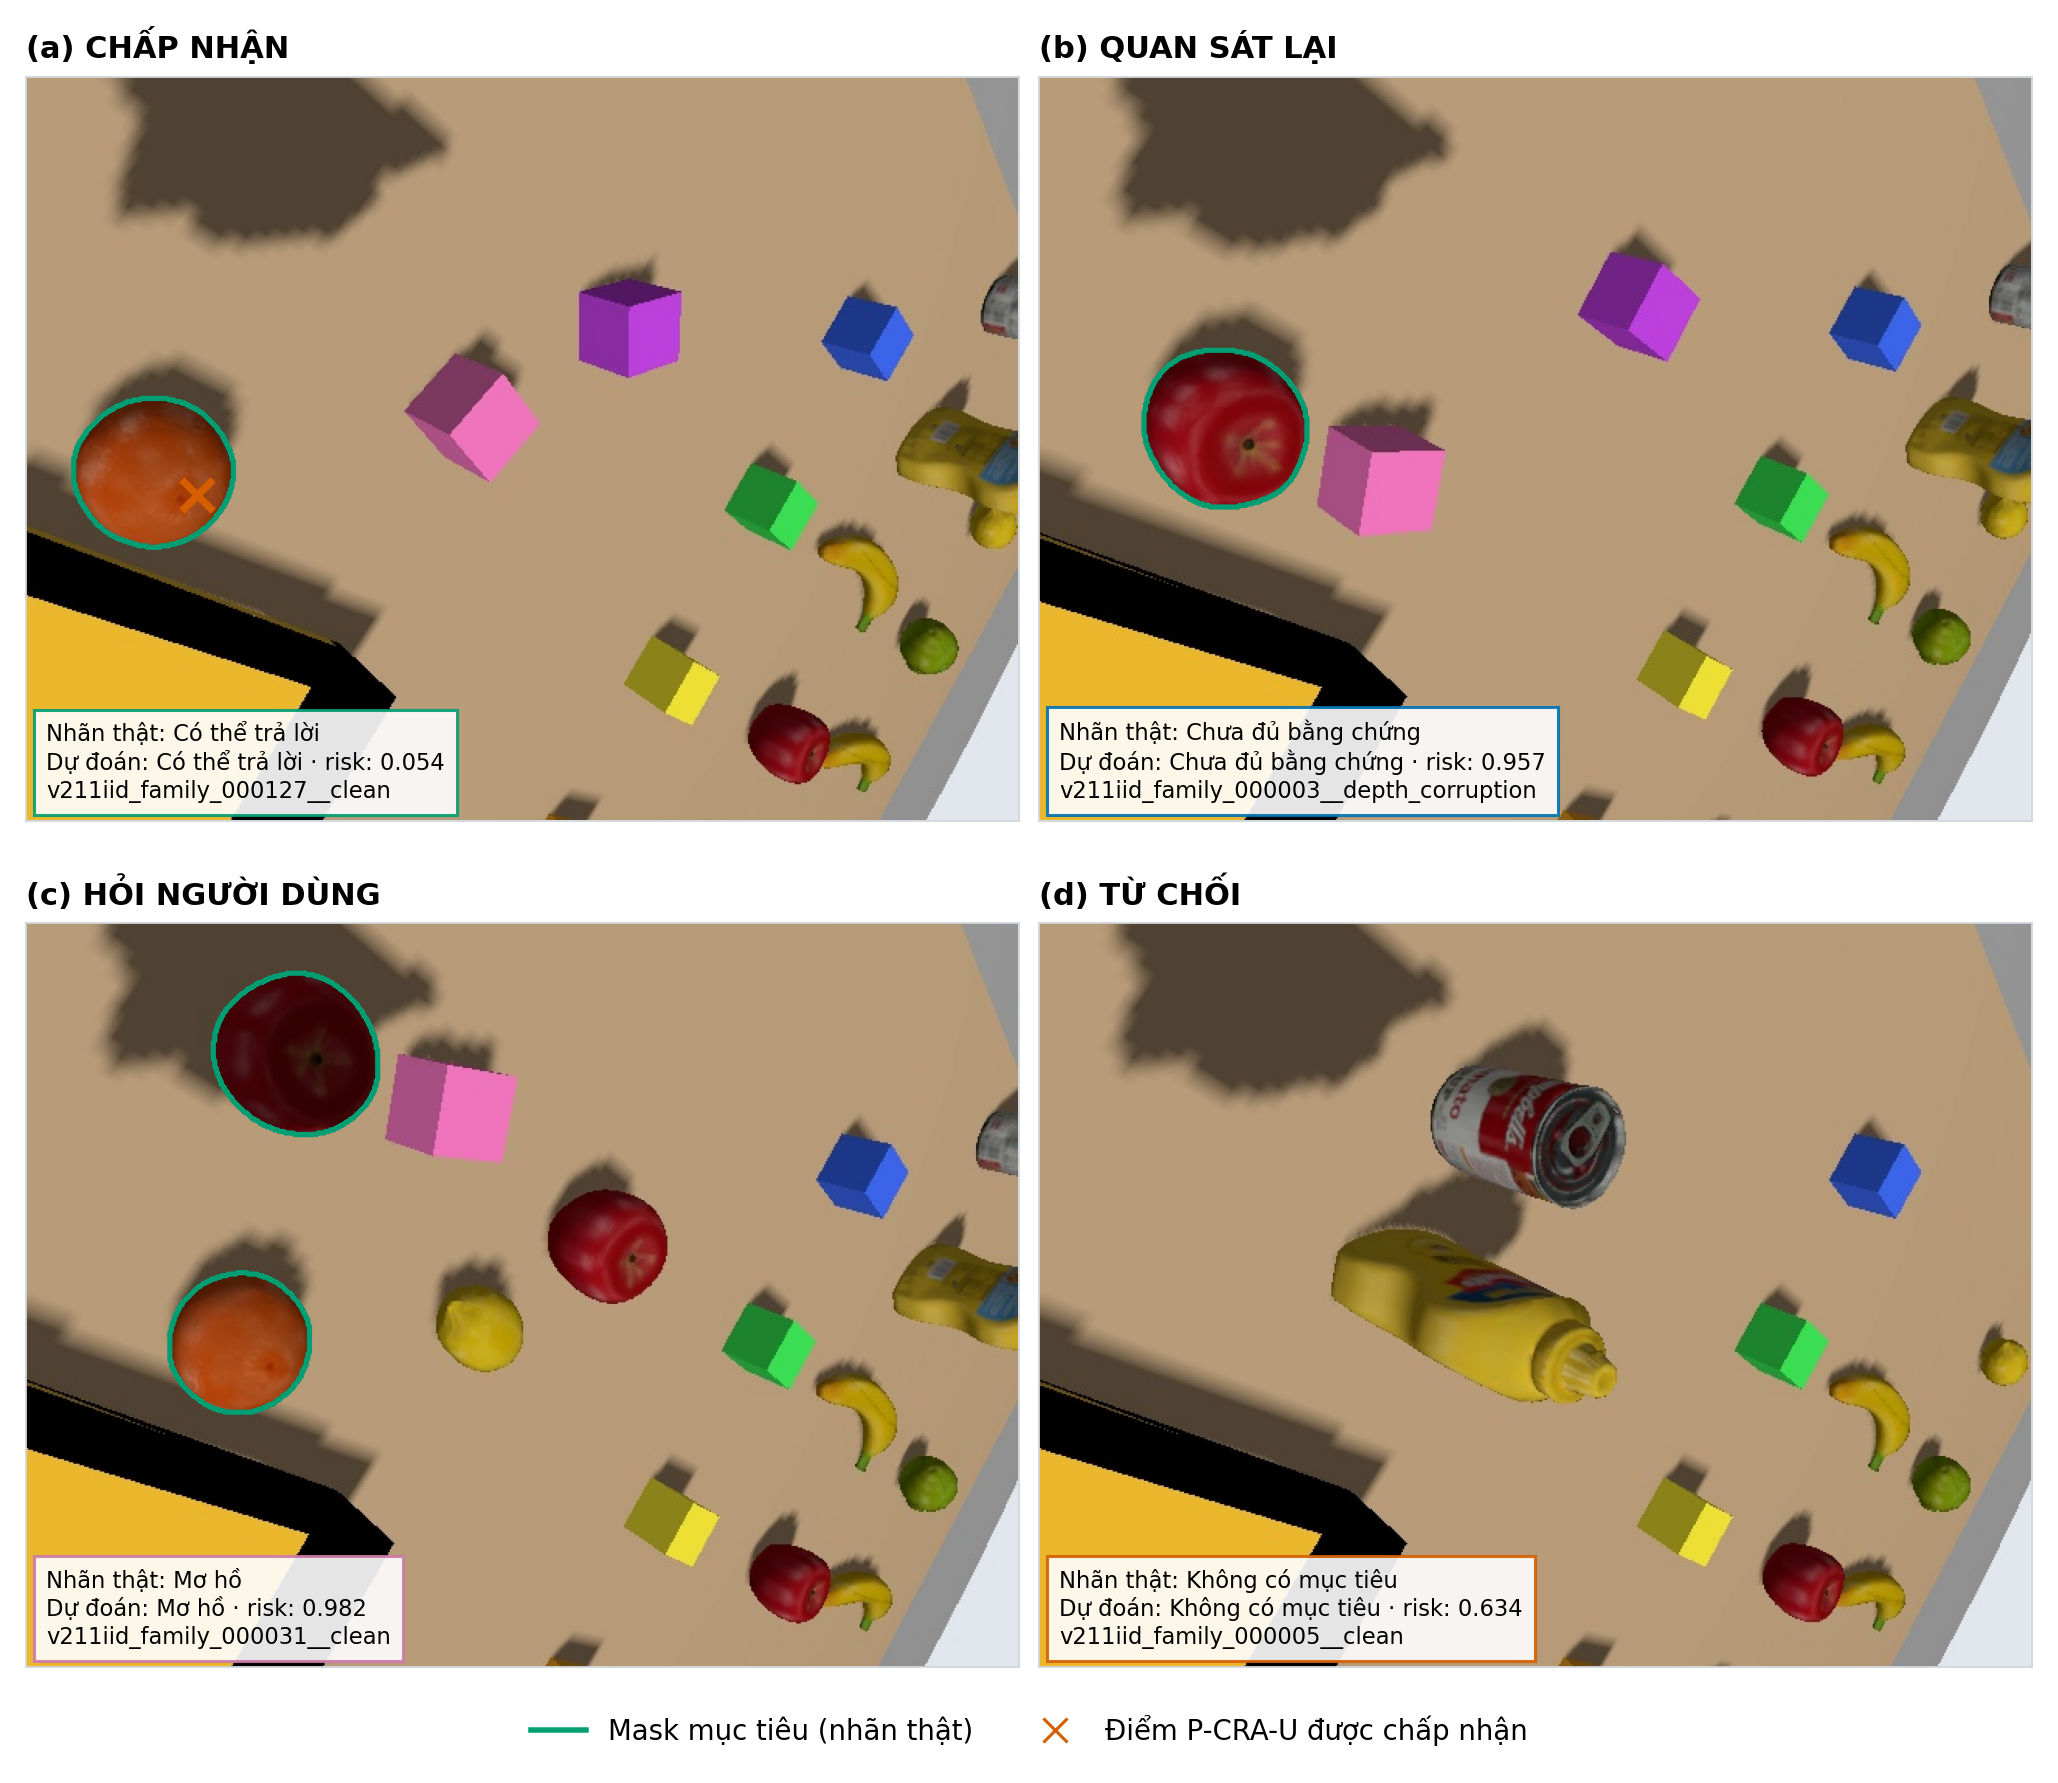
\includegraphics[width=\textwidth]{hinhanh/fig14_four_policy_decisions_adapter_vi.png}
    \caption{Ví dụ thực của bốn quyết định chọn lọc trên RGB Test-IID.
    Đây là kết quả policy từ quan sát tĩnh, không phải bằng chứng
    robot chuyển động hay gắp vật thành công.}
    \label{fig:method-policy-cases}
    {\footnotesize Nguồn: tác giả dựng từ prediction, risk và
    decision Adapter đã lưu trong workspace; ảnh gốc là capture Gazebo.\par}
\end{figure}

\subsection{Giao diện đầu ra và cổng an toàn trước robot}

Decision V2 lưu sample ID, action, reason, risk, threshold, điểm được chọn nếu có, confidence region và source hoạt động. Runtime Adapter lưu action, risk, threshold, predicted answerability và selected point; vùng không gian được ghép từ hậu xử lý nhánh spatial V2 đã khóa, không fit lại bởi logistic33.
Ở V2, source hoạt động là source có score ít nhất 0.5.
Thông tin này phục vụ hiển thị và phân tích, không thay đổi
điểm MAP thành một target khác.

Nếu nối với hệ điều khiển, tầng chấp hành cần có cổng riêng:
\begin{equation}
    \mathrm{allow\_motion}=
    \mathbf{1}[a=\texttt{EXECUTE}]
    \land G_{\mathrm{sensor}}
    \land G_{\mathrm{target}}
    \land G_{\mathrm{temporal}}
    \land G_{\mathrm{geometry}}
    \land G_{\mathrm{planning}}.
\end{equation}
Các $G$ lần lượt đại diện kiểm tra cảm biến, xác nhận vật
đích độc lập, ổn định đa khung hình, hình học và khả năng
lập kế hoạch. Đây là yêu cầu tích hợp hành động, chưa phải
các biến đã được dùng trong hàm \texttt{decide} V2.
Ground-truth của Gazebo chỉ được phép dùng đánh giá sau
dự đoán, không được làm một detector oracle để mở cổng
thực thi mà vẫn báo là hiệu quả của mô hình.

\subsection{Tóm tắt phương pháp và chuyển sang thực nghiệm}

Phương pháp đề xuất bổ sung cho grounding một điểm bằng
biểu diễn target--anchor theo truy vấn, phân bố vị trí,
answerability, source uncertainty và calibrated risk.
RoboRefer được đóng băng; sidecar học đa nhiệm; calibrator
được fit sau cùng trên dữ liệu riêng; và policy sử dụng
các đầu ra đã đóng băng để đưa ra quyết định.

Các thành phần đã hiện thực hóa gồm query slot có ngữ cảnh,
fusion có điều kiện quan hệ bằng MLP/gate, các spatial head,
edge head với nhãn proxy, hai head phân loại, logistic
calibration, vùng highest-density và policy bốn decision.
Parser noun--relation hoàn chỉnh, kiểm chứng cạnh bằng metric
geometry và vòng pick-and-place đã xác minh vẫn cần được
phân biệt với kết quả grounding trên ảnh.

Chương tiếp theo trình bày cách tổ chức dữ liệu theo family,
pipeline capture/cache, môi trường huấn luyện và quy trình
đánh giá. Các so sánh định lượng, bootstrap theo family,
reliability diagram, risk--coverage curve và phân tích lỗi
được dành cho chương kết quả để không trộn thiết kế phương
pháp với bằng chứng hiệu quả thực nghiệm.
